\documentclass[1p]{elsarticle_modified}
%\bibliographystyle{elsarticle-num}

%\usepackage[colorlinks]{hyperref}
%\usepackage{abbrmath_seonhwa} %\Abb, \Ascr, \Acal ,\Abf, \Afrak
\usepackage{amsfonts}
\usepackage{amssymb}
\usepackage{amsmath}
\usepackage{amsthm}
\usepackage{scalefnt}
\usepackage{amsbsy}
\usepackage{kotex}
\usepackage{caption}
\usepackage{subfig}
\usepackage{color}
\usepackage{graphicx}
\usepackage{xcolor} %% white, black, red, green, blue, cyan, magenta, yellow
\usepackage{float}
\usepackage{setspace}
\usepackage{hyperref}

\usepackage{tikz}
\usetikzlibrary{arrows}

\usepackage{multirow}
\usepackage{array} % fixed length table
\usepackage{hhline}

%%%%%%%%%%%%%%%%%%%%%
\makeatletter
\renewcommand*\env@matrix[1][\arraystretch]{%
	\edef\arraystretch{#1}%
	\hskip -\arraycolsep
	\let\@ifnextchar\new@ifnextchar
	\array{*\c@MaxMatrixCols c}}
\makeatother %https://tex.stackexchange.com/questions/14071/how-can-i-increase-the-line-spacing-in-a-matrix
%%%%%%%%%%%%%%%

\usepackage[normalem]{ulem}

\newcommand{\msout}[1]{\ifmmode\text{\sout{\ensuremath{#1}}}\else\sout{#1}\fi}
%SOURCE: \msout is \stkout macro in https://tex.stackexchange.com/questions/20609/strikeout-in-math-mode

\newcommand{\cancel}[1]{
	\ifmmode
	{\color{red}\msout{#1}}
	\else
	{\color{red}\sout{#1}}
	\fi
}

\newcommand{\add}[1]{
	{\color{blue}\uwave{#1}}
}

\newcommand{\replace}[2]{
	\ifmmode
	{\color{red}\msout{#1}}{\color{blue}\uwave{#2}}
	\else
	{\color{red}\sout{#1}}{\color{blue}\uwave{#2}}
	\fi
}

\newcommand{\Sol}{\mathcal{S}} %segment
\newcommand{\D}{D} %diagram
\newcommand{\A}{\mathcal{A}} %arc


%%%%%%%%%%%%%%%%%%%%%%%%%%%%%5 test

\def\sl{\operatorname{\textup{SL}}(2,\Cbb)}
\def\psl{\operatorname{\textup{PSL}}(2,\Cbb)}
\def\quan{\mkern 1mu \triangleright \mkern 1mu}

\theoremstyle{definition}
\newtheorem{thm}{Theorem}[section]
\newtheorem{prop}[thm]{Proposition}
\newtheorem{lem}[thm]{Lemma}
\newtheorem{ques}[thm]{Question}
\newtheorem{cor}[thm]{Corollary}
\newtheorem{defn}[thm]{Definition}
\newtheorem{exam}[thm]{Example}
\newtheorem{rmk}[thm]{Remark}
\newtheorem{alg}[thm]{Algorithm}

\newcommand{\I}{\sqrt{-1}}
\begin{document}

%\begin{frontmatter}
%
%\title{Boundary parabolic representations of knots up to 8 crossings}
%
%%% Group authors per affiliation:
%\author{Yunhi Cho} 
%\address{Department of Mathematics, University of Seoul, Seoul, Korea}
%\ead{yhcho@uos.ac.kr}
%
%
%\author{Seonhwa Kim} %\fnref{s_kim}}
%\address{Center for Geometry and Physics, Institute for Basic Science, Pohang, 37673, Korea}
%\ead{ryeona17@ibs.re.kr}
%
%\author{Hyuk Kim}
%\address{Department of Mathematical Sciences, Seoul National University, Seoul 08826, Korea}
%\ead{hyukkim@snu.ac.kr}
%
%\author{Seokbeom Yoon}
%\address{Department of Mathematical Sciences, Seoul National University, Seoul, 08826,  Korea}
%\ead{sbyoon15@snu.ac.kr}
%
%\begin{abstract}
%We find all boundary parabolic representation of knots up to 8 crossings.
%
%\end{abstract}
%\begin{keyword}
%    \MSC[2010] 57M25 
%\end{keyword}
%
%\end{frontmatter}

%\linenumbers
%\tableofcontents
%
\newcommand\colored[1]{\textcolor{white}{\rule[-0.35ex]{0.8em}{1.4ex}}\kern-0.8em\color{red} #1}%
%\newcommand\colored[1]{\textcolor{white}{ #1}\kern-2.17ex	\textcolor{white}{ #1}\kern-1.81ex	\textcolor{white}{ #1}\kern-2.15ex\color{red}#1	}

{\Large $\underline{12a_{0914}~(K12a_{0914})}$}

\setlength{\tabcolsep}{10pt}
\renewcommand{\arraystretch}{1.6}
\vspace{1cm}\begin{tabular}{m{100pt}>{\centering\arraybackslash}m{274pt}}
\multirow{5}{120pt}{
	\centering
	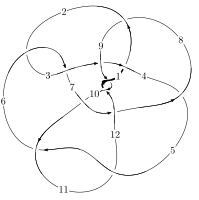
\includegraphics[width=112pt]{../../../GIT/diagram.site/Diagrams/png/1715_12a_0914.png}\\
\ \ \ A knot diagram\footnotemark}&
\allowdisplaybreaks
\textbf{Linearized knot diagam} \\
\cline{2-2}
 &
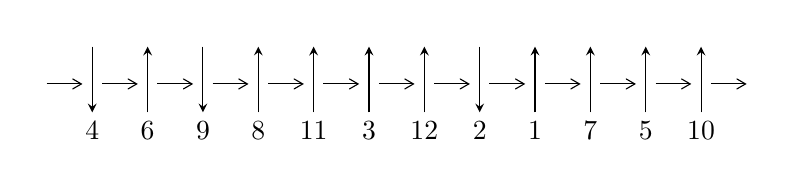
\begin{tikzpicture}[x=20pt, y=17pt]
	% nodes
	\node (C0) at (0, 0) {};
	\node (C1) at (1, 0) {};
	\node (C1U) at (1, +1) {};
	\node (C1D) at (1, -1) {4};

	\node (C2) at (2, 0) {};
	\node (C2U) at (2, +1) {};
	\node (C2D) at (2, -1) {6};

	\node (C3) at (3, 0) {};
	\node (C3U) at (3, +1) {};
	\node (C3D) at (3, -1) {9};

	\node (C4) at (4, 0) {};
	\node (C4U) at (4, +1) {};
	\node (C4D) at (4, -1) {8};

	\node (C5) at (5, 0) {};
	\node (C5U) at (5, +1) {};
	\node (C5D) at (5, -1) {11};

	\node (C6) at (6, 0) {};
	\node (C6U) at (6, +1) {};
	\node (C6D) at (6, -1) {3};

	\node (C7) at (7, 0) {};
	\node (C7U) at (7, +1) {};
	\node (C7D) at (7, -1) {12};

	\node (C8) at (8, 0) {};
	\node (C8U) at (8, +1) {};
	\node (C8D) at (8, -1) {2};

	\node (C9) at (9, 0) {};
	\node (C9U) at (9, +1) {};
	\node (C9D) at (9, -1) {1};

	\node (C10) at (10, 0) {};
	\node (C10U) at (10, +1) {};
	\node (C10D) at (10, -1) {7};

	\node (C11) at (11, 0) {};
	\node (C11U) at (11, +1) {};
	\node (C11D) at (11, -1) {5};

	\node (C12) at (12, 0) {};
	\node (C12U) at (12, +1) {};
	\node (C12D) at (12, -1) {10};
	\node (C13) at (13, 0) {};

	% arrows
	\draw[->,>={angle 60}]
	(C0) edge (C1) (C1) edge (C2) (C2) edge (C3) (C3) edge (C4) (C4) edge (C5) (C5) edge (C6) (C6) edge (C7) (C7) edge (C8) (C8) edge (C9) (C9) edge (C10) (C10) edge (C11) (C11) edge (C12) (C12) edge (C13) ;	\draw[->,>=stealth]
	(C1U) edge (C1D) (C2D) edge (C2U) (C3U) edge (C3D) (C4D) edge (C4U) (C5D) edge (C5U) (C6D) edge (C6U) (C7D) edge (C7U) (C8U) edge (C8D) (C9D) edge (C9U) (C10D) edge (C10U) (C11D) edge (C11U) (C12D) edge (C12U) ;
	\end{tikzpicture} \\
\hhline{~~} \\& 
\textbf{Solving Sequence} \\ \cline{2-2} 
 &
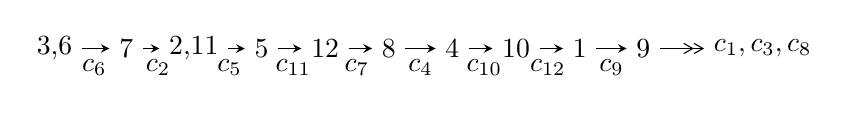
\begin{tikzpicture}[x=23pt, y=7pt]
	% node
	\node (A0) at (-1/8, 0) {3,6};
	\node (A1) at (1, 0) {7};
	\node (A2) at (33/16, 0) {2,11};
	\node (A3) at (25/8, 0) {5};
	\node (A4) at (33/8, 0) {12};
	\node (A5) at (41/8, 0) {8};
	\node (A6) at (49/8, 0) {4};
	\node (A7) at (57/8, 0) {10};
	\node (A8) at (65/8, 0) {1};
	\node (A9) at (73/8, 0) {9};
	\node (C1) at (1/2, -1) {$c_{6}$};
	\node (C2) at (3/2, -1) {$c_{2}$};
	\node (C3) at (21/8, -1) {$c_{5}$};
	\node (C4) at (29/8, -1) {$c_{11}$};
	\node (C5) at (37/8, -1) {$c_{7}$};
	\node (C6) at (45/8, -1) {$c_{4}$};
	\node (C7) at (53/8, -1) {$c_{10}$};
	\node (C8) at (61/8, -1) {$c_{12}$};
	\node (C9) at (69/8, -1) {$c_{9}$};
	\node (A10) at (11, 0) {$c_{1},c_{3},c_{8}$};

	% edge
	\draw[->,>=stealth]	
	(A0) edge (A1) (A1) edge (A2) (A2) edge (A3) (A3) edge (A4) (A4) edge (A5) (A5) edge (A6) (A6) edge (A7) (A7) edge (A8) (A8) edge (A9) ;
	\draw[->>,>={angle 60}]	
	(A9) edge (A10);
\end{tikzpicture} \\ 

\end{tabular} \\

\footnotetext{
The image of knot diagram is generated by the software ``\textbf{Draw programme}" developed by Andrew Bartholomew(\url{http://www.layer8.co.uk/maths/draw/index.htm\#Running-draw}), where we modified some parts for our purpose(\url{https://github.com/CATsTAILs/LinksPainter}).
}\phantom \\ \newline 
\centering \textbf{Ideals for irreducible components\footnotemark of $X_{\text{par}}$} 
 
\begin{align*}
I^u_{1}&=\langle 
6.28945\times10^{1120} u^{177}+3.30828\times10^{1120} u^{176}+\cdots+3.69271\times10^{1123} b+1.15920\times10^{1124},\\
\phantom{I^u_{1}}&\phantom{= \langle  }-4.00966\times10^{1124} u^{177}+3.02679\times10^{1124} u^{176}+\cdots+2.68460\times10^{1126} a-2.52671\times10^{1126},\\
\phantom{I^u_{1}}&\phantom{= \langle  }u^{178}-42 u^{176}+\cdots-9456 u-727\rangle \\
I^u_{2}&=\langle 
-1.53640\times10^{55} u^{50}-3.87380\times10^{55} u^{49}+\cdots+1.01569\times10^{52} b+3.06717\times10^{55},\\
\phantom{I^u_{2}}&\phantom{= \langle  }4.87270\times10^{55} u^{50}+1.19332\times10^{56} u^{49}+\cdots+1.01569\times10^{52} a-8.34046\times10^{55},\;u^{51}+3 u^{50}+\cdots-4 u-1\rangle \\
\\
\end{align*}
\raggedright * 2 irreducible components of $\dim_{\mathbb{C}}=0$, with total 229 representations.\\
\footnotetext{All coefficients of polynomials are rational numbers. But the coefficients are sometimes approximated in decimal forms when there is not enough margin.}
\newpage
\renewcommand{\arraystretch}{1}
\centering \section*{I. $I^u_{1}= \langle 6.29\times10^{1120} u^{177}+3.31\times10^{1120} u^{176}+\cdots+3.69\times10^{1123} b+1.16\times10^{1124},\;-4.01\times10^{1124} u^{177}+3.03\times10^{1124} u^{176}+\cdots+2.68\times10^{1126} a-2.53\times10^{1126},\;u^{178}-42 u^{176}+\cdots-9456 u-727 \rangle$}
\flushleft \textbf{(i) Arc colorings}\\
\begin{tabular}{m{7pt} m{180pt} m{7pt} m{180pt} }
\flushright $a_{3}=$&$\begin{pmatrix}0\\u\end{pmatrix}$ \\
\flushright $a_{6}=$&$\begin{pmatrix}1\\0\end{pmatrix}$ \\
\flushright $a_{7}=$&$\begin{pmatrix}1\\- u^2\end{pmatrix}$ \\
\flushright $a_{2}=$&$\begin{pmatrix}- u\\u\end{pmatrix}$ \\
\flushright $a_{11}=$&$\begin{pmatrix}0.0149358 u^{177}-0.0112746 u^{176}+\cdots-51.2712 u+0.941186\\-0.00170321 u^{177}-0.000895896 u^{176}+\cdots+8.48698 u-3.13915\end{pmatrix}$ \\
\flushright $a_{5}=$&$\begin{pmatrix}-0.00483437 u^{177}+0.00344005 u^{176}+\cdots+89.7759 u+16.1715\\-0.0108380 u^{177}+0.00366179 u^{176}+\cdots+223.707 u+18.2334\end{pmatrix}$ \\
\flushright $a_{12}=$&$\begin{pmatrix}0.00222129 u^{177}-0.00327035 u^{176}+\cdots-54.5037 u-8.44973\\-0.0135021 u^{177}+0.00556319 u^{176}+\cdots+317.850 u+34.3124\end{pmatrix}$ \\
\flushright $a_{8}=$&$\begin{pmatrix}0.0143040 u^{177}-0.000899404 u^{176}+\cdots-563.005 u-69.6296\\0.00417733 u^{177}-0.00495239 u^{176}+\cdots+100.248 u+23.4775\end{pmatrix}$ \\
\flushright $a_{4}=$&$\begin{pmatrix}-0.0216072 u^{177}+0.00944757 u^{176}+\cdots+570.318 u+51.1929\\0.0147707 u^{177}-0.00294898 u^{176}+\cdots-562.222 u-60.1550\end{pmatrix}$ \\
\flushright $a_{10}=$&$\begin{pmatrix}0.0101121 u^{177}-0.00862272 u^{176}+\cdots+35.9964 u+12.2770\\-0.0000760491 u^{177}-0.00120178 u^{176}+\cdots-13.0826 u-5.06709\end{pmatrix}$ \\
\flushright $a_{1}=$&$\begin{pmatrix}0.0120824 u^{177}-0.000905418 u^{176}+\cdots-335.404 u-27.8449\\-0.0108050 u^{177}+0.00165084 u^{176}+\cdots+369.418 u+38.8534\end{pmatrix}$ \\
\flushright $a_{9}=$&$\begin{pmatrix}0.0134274 u^{177}-0.00115207 u^{176}+\cdots-521.107 u-65.3754\\0.00505391 u^{177}-0.00469973 u^{176}+\cdots+58.3488 u+19.2233\end{pmatrix}$\\&\end{tabular}
\flushleft \textbf{(ii) Obstruction class $= -1$}\\~\\
\flushleft \textbf{(iii) Cusp Shapes $= -0.0300055 u^{177}-0.0175349 u^{176}+\cdots+1810.06 u+228.305$}\\~\\
\newpage\renewcommand{\arraystretch}{1}
\flushleft \textbf{(iv) u-Polynomials at the component}\newline \\
\begin{tabular}{m{50pt}|m{274pt}}
Crossings & \hspace{64pt}u-Polynomials at each crossing \\
\hline $$\begin{aligned}c_{1}\end{aligned}$$&$\begin{aligned}
&u^{178}-11 u^{177}+\cdots+484886 u+16630
\end{aligned}$\\
\hline $$\begin{aligned}c_{2},c_{6}\end{aligned}$$&$\begin{aligned}
&u^{178}-42 u^{176}+\cdots-9456 u-727
\end{aligned}$\\
\hline $$\begin{aligned}c_{3}\end{aligned}$$&$\begin{aligned}
&u^{178}-3 u^{177}+\cdots-6074908 u+521284
\end{aligned}$\\
\hline $$\begin{aligned}c_{4}\end{aligned}$$&$\begin{aligned}
&u^{178}-5 u^{177}+\cdots-534111527848 u+12234606751
\end{aligned}$\\
\hline $$\begin{aligned}c_{5},c_{11}\end{aligned}$$&$\begin{aligned}
&u^{178}+u^{177}+\cdots-79956 u-25406
\end{aligned}$\\
\hline $$\begin{aligned}c_{7}\end{aligned}$$&$\begin{aligned}
&u^{178}-11 u^{177}+\cdots+10511353546 u+2936241116
\end{aligned}$\\
\hline $$\begin{aligned}c_{8}\end{aligned}$$&$\begin{aligned}
&u^{178}+4 u^{177}+\cdots-162199 u+18811
\end{aligned}$\\
\hline $$\begin{aligned}c_{9},c_{12}\end{aligned}$$&$\begin{aligned}
&u^{178}+10 u^{177}+\cdots+51945823 u+3103757
\end{aligned}$\\
\hline $$\begin{aligned}c_{10}\end{aligned}$$&$\begin{aligned}
&u^{178}-2 u^{177}+\cdots+7464600509 u+1577563033
\end{aligned}$\\
\hline
\end{tabular}\\~\\
\newpage\renewcommand{\arraystretch}{1}
\flushleft \textbf{(v) Riley Polynomials at the component}\newline \\
\begin{tabular}{m{50pt}|m{274pt}}
Crossings & \hspace{64pt}Riley Polynomials at each crossing \\
\hline $$\begin{aligned}c_{1}\end{aligned}$$&$\begin{aligned}
&y^{178}-37 y^{177}+\cdots-272210308796 y+276556900
\end{aligned}$\\
\hline $$\begin{aligned}c_{2},c_{6}\end{aligned}$$&$\begin{aligned}
&y^{178}-84 y^{177}+\cdots-43018796 y+528529
\end{aligned}$\\
\hline $$\begin{aligned}c_{3}\end{aligned}$$&$\begin{aligned}
&y^{178}-51 y^{177}+\cdots-21326040167832 y+271737008656
\end{aligned}$\\
\hline $$\begin{aligned}c_{4}\end{aligned}$$&$\begin{aligned}
&y^{178}+99 y^{177}+\cdots-4.90\times10^{23} y+1.50\times10^{20}
\end{aligned}$\\
\hline $$\begin{aligned}c_{5},c_{11}\end{aligned}$$&$\begin{aligned}
&y^{178}+121 y^{177}+\cdots+19611196928 y+645464836
\end{aligned}$\\
\hline $$\begin{aligned}c_{7}\end{aligned}$$&$\begin{aligned}
&y^{178}+59 y^{177}+\cdots+4.34\times10^{20} y+8.62\times10^{18}
\end{aligned}$\\
\hline $$\begin{aligned}c_{8}\end{aligned}$$&$\begin{aligned}
&y^{178}-26 y^{177}+\cdots-35205027563 y+353853721
\end{aligned}$\\
\hline $$\begin{aligned}c_{9},c_{12}\end{aligned}$$&$\begin{aligned}
&y^{178}+150 y^{177}+\cdots-369428626219007 y+9633307515049
\end{aligned}$\\
\hline $$\begin{aligned}c_{10}\end{aligned}$$&$\begin{aligned}
&y^{178}+62 y^{177}+\cdots+6.12\times10^{19} y+2.49\times10^{18}
\end{aligned}$\\
\hline
\end{tabular}\\~\\
\newpage\flushleft \textbf{(vi) Complex Volumes and Cusp Shapes}
$$\begin{array}{c|c|c}  
\text{Solutions to }I^u_{1}& \I (\text{vol} + \sqrt{-1}CS) & \text{Cusp shape}\\
 \hline 
\begin{aligned}
u &= -0.947667 + 0.379567 I \\
a &= \phantom{-}1.42134 - 0.60528 I \\
b &= -0.014422 + 1.121210 I\end{aligned}
 & -3.38009 - 1.54141 I & \phantom{-0.000000 } 0 \\ \hline\begin{aligned}
u &= -0.947667 - 0.379567 I \\
a &= \phantom{-}1.42134 + 0.60528 I \\
b &= -0.014422 - 1.121210 I\end{aligned}
 & -3.38009 + 1.54141 I & \phantom{-0.000000 } 0 \\ \hline\begin{aligned}
u &= \phantom{-}0.926334 + 0.444741 I \\
a &= \phantom{-}1.50332 - 0.69935 I \\
b &= -0.697530 + 0.601342 I\end{aligned}
 & -1.56305 + 6.11918 I & \phantom{-0.000000 } 0 \\ \hline\begin{aligned}
u &= \phantom{-}0.926334 - 0.444741 I \\
a &= \phantom{-}1.50332 + 0.69935 I \\
b &= -0.697530 - 0.601342 I\end{aligned}
 & -1.56305 - 6.11918 I & \phantom{-0.000000 } 0 \\ \hline\begin{aligned}
u &= \phantom{-}0.809819 + 0.632534 I \\
a &= -0.445712 - 0.596758 I \\
b &= -0.68310 + 1.53067 I\end{aligned}
 & -6.47665 - 0.76175 I & \phantom{-0.000000 } 0 \\ \hline\begin{aligned}
u &= \phantom{-}0.809819 - 0.632534 I \\
a &= -0.445712 + 0.596758 I \\
b &= -0.68310 - 1.53067 I\end{aligned}
 & -6.47665 + 0.76175 I & \phantom{-0.000000 } 0 \\ \hline\begin{aligned}
u &= \phantom{-}0.924597 + 0.473780 I \\
a &= \phantom{-}1.91212 + 0.18474 I \\
b &= \phantom{-}0.060030 - 1.042480 I\end{aligned}
 & -2.96311 - 2.56203 I & \phantom{-0.000000 } 0 \\ \hline\begin{aligned}
u &= \phantom{-}0.924597 - 0.473780 I \\
a &= \phantom{-}1.91212 - 0.18474 I \\
b &= \phantom{-}0.060030 + 1.042480 I\end{aligned}
 & -2.96311 + 2.56203 I & \phantom{-0.000000 } 0 \\ \hline\begin{aligned}
u &= \phantom{-}0.449068 + 0.944421 I \\
a &= \phantom{-}0.128688 - 0.325894 I \\
b &= \phantom{-}0.46742 - 1.36176 I\end{aligned}
 & -4.70991 - 8.60785 I & \phantom{-0.000000 } 0 \\ \hline\begin{aligned}
u &= \phantom{-}0.449068 - 0.944421 I \\
a &= \phantom{-}0.128688 + 0.325894 I \\
b &= \phantom{-}0.46742 + 1.36176 I\end{aligned}
 & -4.70991 + 8.60785 I & \phantom{-0.000000 } 0\\
 \hline 
 \end{array}$$\newpage$$\begin{array}{c|c|c}  
\text{Solutions to }I^u_{1}& \I (\text{vol} + \sqrt{-1}CS) & \text{Cusp shape}\\
 \hline 
\begin{aligned}
u &= \phantom{-}0.924161 + 0.517314 I \\
a &= -2.25069 - 0.15388 I \\
b &= \phantom{-}0.50604 + 1.44308 I\end{aligned}
 & -4.09570 + 3.29574 I & \phantom{-0.000000 } 0 \\ \hline\begin{aligned}
u &= \phantom{-}0.924161 - 0.517314 I \\
a &= -2.25069 + 0.15388 I \\
b &= \phantom{-}0.50604 - 1.44308 I\end{aligned}
 & -4.09570 - 3.29574 I & \phantom{-0.000000 } 0 \\ \hline\begin{aligned}
u &= -1.060090 + 0.016903 I \\
a &= -1.54719 - 0.15027 I \\
b &= \phantom{-}0.634517 - 0.460967 I\end{aligned}
 & \phantom{-}4.33491 + 0.24862 I & \phantom{-0.000000 } 0 \\ \hline\begin{aligned}
u &= -1.060090 - 0.016903 I \\
a &= -1.54719 + 0.15027 I \\
b &= \phantom{-}0.634517 + 0.460967 I\end{aligned}
 & \phantom{-}4.33491 - 0.24862 I & \phantom{-0.000000 } 0 \\ \hline\begin{aligned}
u &= \phantom{-}0.836311 + 0.419010 I \\
a &= \phantom{-}0.38767 - 1.37963 I \\
b &= -0.147077 - 1.297050 I\end{aligned}
 & -3.31973 + 6.22541 I & \phantom{-0.000000 } 0 \\ \hline\begin{aligned}
u &= \phantom{-}0.836311 - 0.419010 I \\
a &= \phantom{-}0.38767 + 1.37963 I \\
b &= -0.147077 + 1.297050 I\end{aligned}
 & -3.31973 - 6.22541 I & \phantom{-0.000000 } 0 \\ \hline\begin{aligned}
u &= -0.808382 + 0.700683 I \\
a &= \phantom{-}1.44536 + 0.90906 I \\
b &= -0.252204 + 0.781227 I\end{aligned}
 & -3.25871 - 5.80862 I & \phantom{-0.000000 } 0 \\ \hline\begin{aligned}
u &= -0.808382 - 0.700683 I \\
a &= \phantom{-}1.44536 - 0.90906 I \\
b &= -0.252204 - 0.781227 I\end{aligned}
 & -3.25871 + 5.80862 I & \phantom{-0.000000 } 0 \\ \hline\begin{aligned}
u &= \phantom{-}0.781314 + 0.496599 I \\
a &= -0.449043 - 0.076592 I \\
b &= -0.32539 + 1.60708 I\end{aligned}
 & -4.58588 + 0.84097 I & \phantom{-0.000000 } 0 \\ \hline\begin{aligned}
u &= \phantom{-}0.781314 - 0.496599 I \\
a &= -0.449043 + 0.076592 I \\
b &= -0.32539 - 1.60708 I\end{aligned}
 & -4.58588 - 0.84097 I & \phantom{-0.000000 } 0\\
 \hline 
 \end{array}$$\newpage$$\begin{array}{c|c|c}  
\text{Solutions to }I^u_{1}& \I (\text{vol} + \sqrt{-1}CS) & \text{Cusp shape}\\
 \hline 
\begin{aligned}
u &= \phantom{-}1.058190 + 0.191699 I \\
a &= \phantom{-}1.08570 - 1.00416 I \\
b &= -0.701552 + 0.319777 I\end{aligned}
 & -1.079410 - 0.575584 I & \phantom{-0.000000 } 0 \\ \hline\begin{aligned}
u &= \phantom{-}1.058190 - 0.191699 I \\
a &= \phantom{-}1.08570 + 1.00416 I \\
b &= -0.701552 - 0.319777 I\end{aligned}
 & -1.079410 + 0.575584 I & \phantom{-0.000000 } 0 \\ \hline\begin{aligned}
u &= \phantom{-}0.972245 + 0.470105 I \\
a &= \phantom{-}1.51111 - 0.65538 I \\
b &= -1.082680 + 0.199899 I\end{aligned}
 & -3.43359 + 4.61844 I & \phantom{-0.000000 } 0 \\ \hline\begin{aligned}
u &= \phantom{-}0.972245 - 0.470105 I \\
a &= \phantom{-}1.51111 + 0.65538 I \\
b &= -1.082680 - 0.199899 I\end{aligned}
 & -3.43359 - 4.61844 I & \phantom{-0.000000 } 0 \\ \hline\begin{aligned}
u &= -0.954395 + 0.508473 I \\
a &= \phantom{-}0.021135 + 0.544296 I \\
b &= \phantom{-}0.015236 + 0.384864 I\end{aligned}
 & -3.54566 - 1.02725 I & \phantom{-0.000000 } 0 \\ \hline\begin{aligned}
u &= -0.954395 - 0.508473 I \\
a &= \phantom{-}0.021135 - 0.544296 I \\
b &= \phantom{-}0.015236 - 0.384864 I\end{aligned}
 & -3.54566 + 1.02725 I & \phantom{-0.000000 } 0 \\ \hline\begin{aligned}
u &= \phantom{-}0.822117 + 0.402520 I \\
a &= -1.119350 - 0.696683 I \\
b &= \phantom{-}0.609474 + 0.140591 I\end{aligned}
 & -1.96166 - 2.57986 I & \phantom{-0.000000 } 0 \\ \hline\begin{aligned}
u &= \phantom{-}0.822117 - 0.402520 I \\
a &= -1.119350 + 0.696683 I \\
b &= \phantom{-}0.609474 - 0.140591 I\end{aligned}
 & -1.96166 + 2.57986 I & \phantom{-0.000000 } 0 \\ \hline\begin{aligned}
u &= \phantom{-}0.898887 + 0.611419 I \\
a &= -1.97910 + 0.36133 I \\
b &= \phantom{-}0.87473 + 1.44747 I\end{aligned}
 & -6.19054 + 5.63955 I & \phantom{-0.000000 } 0 \\ \hline\begin{aligned}
u &= \phantom{-}0.898887 - 0.611419 I \\
a &= -1.97910 - 0.36133 I \\
b &= \phantom{-}0.87473 - 1.44747 I\end{aligned}
 & -6.19054 - 5.63955 I & \phantom{-0.000000 } 0\\
 \hline 
 \end{array}$$\newpage$$\begin{array}{c|c|c}  
\text{Solutions to }I^u_{1}& \I (\text{vol} + \sqrt{-1}CS) & \text{Cusp shape}\\
 \hline 
\begin{aligned}
u &= -0.380457 + 1.031100 I \\
a &= \phantom{-}0.402217 + 0.710582 I \\
b &= -0.976391 + 0.004940 I\end{aligned}
 & -6.45632 + 8.43471 I & \phantom{-0.000000 } 0 \\ \hline\begin{aligned}
u &= -0.380457 - 1.031100 I \\
a &= \phantom{-}0.402217 - 0.710582 I \\
b &= -0.976391 - 0.004940 I\end{aligned}
 & -6.45632 - 8.43471 I & \phantom{-0.000000 } 0 \\ \hline\begin{aligned}
u &= -0.029036 + 1.106290 I \\
a &= -0.714582 - 0.338765 I \\
b &= -0.135825 - 1.067320 I\end{aligned}
 & -9.12938 + 0.59289 I & \phantom{-0.000000 } 0 \\ \hline\begin{aligned}
u &= -0.029036 - 1.106290 I \\
a &= -0.714582 + 0.338765 I \\
b &= -0.135825 + 1.067320 I\end{aligned}
 & -9.12938 - 0.59289 I & \phantom{-0.000000 } 0 \\ \hline\begin{aligned}
u &= -0.956885 + 0.556639 I \\
a &= \phantom{-}1.50918 + 0.71619 I \\
b &= -0.912027 + 0.319180 I\end{aligned}
 & -3.44555 - 6.30338 I & \phantom{-0.000000 } 0 \\ \hline\begin{aligned}
u &= -0.956885 - 0.556639 I \\
a &= \phantom{-}1.50918 - 0.71619 I \\
b &= -0.912027 - 0.319180 I\end{aligned}
 & -3.44555 + 6.30338 I & \phantom{-0.000000 } 0 \\ \hline\begin{aligned}
u &= \phantom{-}0.631351 + 0.631249 I \\
a &= \phantom{-}2.71693 - 0.41430 I \\
b &= -0.546921 - 1.300510 I\end{aligned}
 & -10.33440 - 3.16208 I & \phantom{-0.000000 } 0 \\ \hline\begin{aligned}
u &= \phantom{-}0.631351 - 0.631249 I \\
a &= \phantom{-}2.71693 + 0.41430 I \\
b &= -0.546921 + 1.300510 I\end{aligned}
 & -10.33440 + 3.16208 I & \phantom{-0.000000 } 0 \\ \hline\begin{aligned}
u &= -0.969339 + 0.537826 I \\
a &= -2.07389 + 0.28246 I \\
b &= \phantom{-}0.60288 - 1.28646 I\end{aligned}
 & -3.59585 - 7.82267 I & \phantom{-0.000000 } 0 \\ \hline\begin{aligned}
u &= -0.969339 - 0.537826 I \\
a &= -2.07389 - 0.28246 I \\
b &= \phantom{-}0.60288 + 1.28646 I\end{aligned}
 & -3.59585 + 7.82267 I & \phantom{-0.000000 } 0\\
 \hline 
 \end{array}$$\newpage$$\begin{array}{c|c|c}  
\text{Solutions to }I^u_{1}& \I (\text{vol} + \sqrt{-1}CS) & \text{Cusp shape}\\
 \hline 
\begin{aligned}
u &= \phantom{-}1.048130 + 0.360997 I \\
a &= -1.202110 + 0.624225 I \\
b &= \phantom{-}0.719536 - 0.542905 I\end{aligned}
 & \phantom{-}3.01331 + 2.90550 I & \phantom{-0.000000 } 0 \\ \hline\begin{aligned}
u &= \phantom{-}1.048130 - 0.360997 I \\
a &= -1.202110 - 0.624225 I \\
b &= \phantom{-}0.719536 + 0.542905 I\end{aligned}
 & \phantom{-}3.01331 - 2.90550 I & \phantom{-0.000000 } 0 \\ \hline\begin{aligned}
u &= -0.114827 + 0.882969 I \\
a &= -0.0127833 + 0.0844290 I \\
b &= \phantom{-}0.326135 + 1.328610 I\end{aligned}
 & -9.88982 + 5.35873 I & \phantom{-0.000000 } 0 \\ \hline\begin{aligned}
u &= -0.114827 - 0.882969 I \\
a &= -0.0127833 - 0.0844290 I \\
b &= \phantom{-}0.326135 - 1.328610 I\end{aligned}
 & -9.88982 - 5.35873 I & \phantom{-0.000000 } 0 \\ \hline\begin{aligned}
u &= -1.092470 + 0.198121 I \\
a &= \phantom{-}1.51423 + 0.11291 I \\
b &= -0.950087 + 0.762070 I\end{aligned}
 & \phantom{-}3.36048 - 5.82580 I & \phantom{-0.000000 } 0 \\ \hline\begin{aligned}
u &= -1.092470 - 0.198121 I \\
a &= \phantom{-}1.51423 - 0.11291 I \\
b &= -0.950087 - 0.762070 I\end{aligned}
 & \phantom{-}3.36048 + 5.82580 I & \phantom{-0.000000 } 0 \\ \hline\begin{aligned}
u &= -0.808263 + 0.308054 I \\
a &= \phantom{-}1.26209 + 0.77653 I \\
b &= \phantom{-}0.044147 - 0.482200 I\end{aligned}
 & -4.32456 - 2.55086 I & \phantom{-0.000000 } 0 \\ \hline\begin{aligned}
u &= -0.808263 - 0.308054 I \\
a &= \phantom{-}1.26209 - 0.77653 I \\
b &= \phantom{-}0.044147 + 0.482200 I\end{aligned}
 & -4.32456 + 2.55086 I & \phantom{-0.000000 } 0 \\ \hline\begin{aligned}
u &= -0.655202 + 0.563352 I \\
a &= \phantom{-}0.115464 + 0.119092 I \\
b &= -0.37811 - 1.39811 I\end{aligned}
 & -4.54033 + 3.42006 I & \phantom{-0.000000 } 0 \\ \hline\begin{aligned}
u &= -0.655202 - 0.563352 I \\
a &= \phantom{-}0.115464 - 0.119092 I \\
b &= -0.37811 + 1.39811 I\end{aligned}
 & -4.54033 - 3.42006 I & \phantom{-0.000000 } 0\\
 \hline 
 \end{array}$$\newpage$$\begin{array}{c|c|c}  
\text{Solutions to }I^u_{1}& \I (\text{vol} + \sqrt{-1}CS) & \text{Cusp shape}\\
 \hline 
\begin{aligned}
u &= -1.014490 + 0.530224 I \\
a &= \phantom{-}0.908974 + 0.862160 I \\
b &= -0.131011 + 1.035530 I\end{aligned}
 & -2.27629 + 0.87176 I & \phantom{-0.000000 } 0 \\ \hline\begin{aligned}
u &= -1.014490 - 0.530224 I \\
a &= \phantom{-}0.908974 - 0.862160 I \\
b &= -0.131011 - 1.035530 I\end{aligned}
 & -2.27629 - 0.87176 I & \phantom{-0.000000 } 0 \\ \hline\begin{aligned}
u &= -0.943727 + 0.669146 I \\
a &= -1.082320 - 0.855634 I \\
b &= \phantom{-}0.170005 - 1.013660 I\end{aligned}
 & \phantom{-}1.27616 - 2.63741 I & \phantom{-0.000000 } 0 \\ \hline\begin{aligned}
u &= -0.943727 - 0.669146 I \\
a &= -1.082320 + 0.855634 I \\
b &= \phantom{-}0.170005 + 1.013660 I\end{aligned}
 & \phantom{-}1.27616 + 2.63741 I & \phantom{-0.000000 } 0 \\ \hline\begin{aligned}
u &= \phantom{-}0.751036 + 0.374110 I \\
a &= -1.313110 + 0.523190 I \\
b &= \phantom{-}1.075420 - 0.284539 I\end{aligned}
 & -4.29974 - 0.99331 I & \phantom{-0.000000 } 0 \\ \hline\begin{aligned}
u &= \phantom{-}0.751036 - 0.374110 I \\
a &= -1.313110 - 0.523190 I \\
b &= \phantom{-}1.075420 + 0.284539 I\end{aligned}
 & -4.29974 + 0.99331 I & \phantom{-0.000000 } 0 \\ \hline\begin{aligned}
u &= -1.031050 + 0.537736 I \\
a &= \phantom{-}1.20834 + 0.83176 I \\
b &= -1.42347 - 0.09857 I\end{aligned}
 & \phantom{-}1.84331 - 7.55297 I & \phantom{-0.000000 } 0 \\ \hline\begin{aligned}
u &= -1.031050 - 0.537736 I \\
a &= \phantom{-}1.20834 - 0.83176 I \\
b &= -1.42347 + 0.09857 I\end{aligned}
 & \phantom{-}1.84331 + 7.55297 I & \phantom{-0.000000 } 0 \\ \hline\begin{aligned}
u &= \phantom{-}0.780725 + 0.865884 I \\
a &= -0.828541 + 0.882667 I \\
b &= \phantom{-}0.881199 + 0.534004 I\end{aligned}
 & -1.69298 + 4.69284 I & \phantom{-0.000000 } 0 \\ \hline\begin{aligned}
u &= \phantom{-}0.780725 - 0.865884 I \\
a &= -0.828541 - 0.882667 I \\
b &= \phantom{-}0.881199 - 0.534004 I\end{aligned}
 & -1.69298 - 4.69284 I & \phantom{-0.000000 } 0\\
 \hline 
 \end{array}$$\newpage$$\begin{array}{c|c|c}  
\text{Solutions to }I^u_{1}& \I (\text{vol} + \sqrt{-1}CS) & \text{Cusp shape}\\
 \hline 
\begin{aligned}
u &= \phantom{-}1.111410 + 0.355404 I \\
a &= -0.174586 + 0.661924 I \\
b &= \phantom{-}0.182500 - 0.563894 I\end{aligned}
 & \phantom{-}2.54596 + 0.79149 I & \phantom{-0.000000 } 0 \\ \hline\begin{aligned}
u &= \phantom{-}1.111410 - 0.355404 I \\
a &= -0.174586 - 0.661924 I \\
b &= \phantom{-}0.182500 + 0.563894 I\end{aligned}
 & \phantom{-}2.54596 - 0.79149 I & \phantom{-0.000000 } 0 \\ \hline\begin{aligned}
u &= -0.513117 + 0.653335 I \\
a &= -0.466255 + 0.583888 I \\
b &= -0.282176 - 1.359300 I\end{aligned}
 & -8.92158 + 0.13770 I & \phantom{-0.000000 } 0 \\ \hline\begin{aligned}
u &= -0.513117 - 0.653335 I \\
a &= -0.466255 - 0.583888 I \\
b &= -0.282176 + 1.359300 I\end{aligned}
 & -8.92158 - 0.13770 I & \phantom{-0.000000 } 0 \\ \hline\begin{aligned}
u &= \phantom{-}1.007550 + 0.600676 I \\
a &= -0.025885 + 0.339012 I \\
b &= \phantom{-}0.49191 - 1.56949 I\end{aligned}
 & -9.16806 + 8.02351 I & \phantom{-0.000000 } 0 \\ \hline\begin{aligned}
u &= \phantom{-}1.007550 - 0.600676 I \\
a &= -0.025885 - 0.339012 I \\
b &= \phantom{-}0.49191 + 1.56949 I\end{aligned}
 & -9.16806 - 8.02351 I & \phantom{-0.000000 } 0 \\ \hline\begin{aligned}
u &= \phantom{-}1.154000 + 0.238602 I \\
a &= \phantom{-}1.223730 - 0.260558 I \\
b &= -0.887826 - 0.568921 I\end{aligned}
 & \phantom{-}3.54911 - 0.58151 I & \phantom{-0.000000 } 0 \\ \hline\begin{aligned}
u &= \phantom{-}1.154000 - 0.238602 I \\
a &= \phantom{-}1.223730 + 0.260558 I \\
b &= -0.887826 + 0.568921 I\end{aligned}
 & \phantom{-}3.54911 + 0.58151 I & \phantom{-0.000000 } 0 \\ \hline\begin{aligned}
u &= -0.783587 + 0.244056 I \\
a &= \phantom{-}2.02710 + 0.73020 I \\
b &= -0.354733 + 1.283260 I\end{aligned}
 & -4.33625 - 3.75187 I & \phantom{-0.000000 } 0 \\ \hline\begin{aligned}
u &= -0.783587 - 0.244056 I \\
a &= \phantom{-}2.02710 - 0.73020 I \\
b &= -0.354733 - 1.283260 I\end{aligned}
 & -4.33625 + 3.75187 I & \phantom{-0.000000 } 0\\
 \hline 
 \end{array}$$\newpage$$\begin{array}{c|c|c}  
\text{Solutions to }I^u_{1}& \I (\text{vol} + \sqrt{-1}CS) & \text{Cusp shape}\\
 \hline 
\begin{aligned}
u &= \phantom{-}1.057070 + 0.532257 I \\
a &= \phantom{-}2.41823 - 0.26547 I \\
b &= -0.127009 - 1.143050 I\end{aligned}
 & -6.51880 + 3.49580 I & \phantom{-0.000000 } 0 \\ \hline\begin{aligned}
u &= \phantom{-}1.057070 - 0.532257 I \\
a &= \phantom{-}2.41823 + 0.26547 I \\
b &= -0.127009 + 1.143050 I\end{aligned}
 & -6.51880 - 3.49580 I & \phantom{-0.000000 } 0 \\ \hline\begin{aligned}
u &= \phantom{-}1.082730 + 0.491385 I \\
a &= \phantom{-}1.071400 - 0.544451 I \\
b &= -1.201520 + 0.235263 I\end{aligned}
 & \phantom{-}1.07181 + 1.71954 I & \phantom{-0.000000 } 0 \\ \hline\begin{aligned}
u &= \phantom{-}1.082730 - 0.491385 I \\
a &= \phantom{-}1.071400 + 0.544451 I \\
b &= -1.201520 - 0.235263 I\end{aligned}
 & \phantom{-}1.07181 - 1.71954 I & \phantom{-0.000000 } 0 \\ \hline\begin{aligned}
u &= \phantom{-}0.311847 + 0.748441 I \\
a &= -0.241082 - 0.410147 I \\
b &= \phantom{-}0.27410 - 1.41704 I\end{aligned}
 & -10.69170 - 5.86905 I & \phantom{-0.000000 } 0 \\ \hline\begin{aligned}
u &= \phantom{-}0.311847 - 0.748441 I \\
a &= -0.241082 + 0.410147 I \\
b &= \phantom{-}0.27410 + 1.41704 I\end{aligned}
 & -10.69170 + 5.86905 I & \phantom{-0.000000 } 0 \\ \hline\begin{aligned}
u &= \phantom{-}1.092210 + 0.472786 I \\
a &= -0.82807 + 1.80986 I \\
b &= \phantom{-}0.095846 + 1.264100 I\end{aligned}
 & -6.47257 + 8.92477 I & \phantom{-0.000000 } 0 \\ \hline\begin{aligned}
u &= \phantom{-}1.092210 - 0.472786 I \\
a &= -0.82807 - 1.80986 I \\
b &= \phantom{-}0.095846 - 1.264100 I\end{aligned}
 & -6.47257 - 8.92477 I & \phantom{-0.000000 } 0 \\ \hline\begin{aligned}
u &= -0.691686 + 0.417148 I \\
a &= -0.190947 - 0.812444 I \\
b &= \phantom{-}0.902425 + 0.668823 I\end{aligned}
 & -4.39631 + 2.05619 I & \phantom{-0.000000 } 0 \\ \hline\begin{aligned}
u &= -0.691686 - 0.417148 I \\
a &= -0.190947 + 0.812444 I \\
b &= \phantom{-}0.902425 - 0.668823 I\end{aligned}
 & -4.39631 - 2.05619 I & \phantom{-0.000000 } 0\\
 \hline 
 \end{array}$$\newpage$$\begin{array}{c|c|c}  
\text{Solutions to }I^u_{1}& \I (\text{vol} + \sqrt{-1}CS) & \text{Cusp shape}\\
 \hline 
\begin{aligned}
u &= \phantom{-}1.198360 + 0.042819 I \\
a &= \phantom{-}0.886174 + 0.610418 I \\
b &= -0.627004 - 0.816665 I\end{aligned}
 & \phantom{-}2.86323 - 0.15819 I & \phantom{-0.000000 } 0 \\ \hline\begin{aligned}
u &= \phantom{-}1.198360 - 0.042819 I \\
a &= \phantom{-}0.886174 - 0.610418 I \\
b &= -0.627004 + 0.816665 I\end{aligned}
 & \phantom{-}2.86323 + 0.15819 I & \phantom{-0.000000 } 0 \\ \hline\begin{aligned}
u &= -0.188249 + 0.777185 I \\
a &= \phantom{-}0.413459 - 0.160180 I \\
b &= -0.185165 - 1.030810 I\end{aligned}
 & -1.39804 + 2.57312 I & \phantom{-0.000000 } 0 \\ \hline\begin{aligned}
u &= -0.188249 - 0.777185 I \\
a &= \phantom{-}0.413459 + 0.160180 I \\
b &= -0.185165 + 1.030810 I\end{aligned}
 & -1.39804 - 2.57312 I & \phantom{-0.000000 } 0 \\ \hline\begin{aligned}
u &= -1.028400 + 0.626041 I \\
a &= -1.49423 + 0.10849 I \\
b &= \phantom{-}0.64879 - 1.29451 I\end{aligned}
 & -7.43636 - 5.22012 I & \phantom{-0.000000 } 0 \\ \hline\begin{aligned}
u &= -1.028400 - 0.626041 I \\
a &= -1.49423 - 0.10849 I \\
b &= \phantom{-}0.64879 + 1.29451 I\end{aligned}
 & -7.43636 + 5.22012 I & \phantom{-0.000000 } 0 \\ \hline\begin{aligned}
u &= -0.458954 + 0.649679 I \\
a &= \phantom{-}3.30551 + 0.88960 I \\
b &= -0.485724 + 1.155790 I\end{aligned}
 & -9.24289 - 5.89563 I & \phantom{-0.000000 } 0 \\ \hline\begin{aligned}
u &= -0.458954 - 0.649679 I \\
a &= \phantom{-}3.30551 - 0.88960 I \\
b &= -0.485724 - 1.155790 I\end{aligned}
 & -9.24289 + 5.89563 I & \phantom{-0.000000 } 0 \\ \hline\begin{aligned}
u &= -0.769276 + 0.938958 I \\
a &= \phantom{-}0.231990 + 0.161515 I \\
b &= \phantom{-}0.154553 + 1.028400 I\end{aligned}
 & -3.76430 - 0.56463 I & \phantom{-0.000000 } 0 \\ \hline\begin{aligned}
u &= -0.769276 - 0.938958 I \\
a &= \phantom{-}0.231990 - 0.161515 I \\
b &= \phantom{-}0.154553 - 1.028400 I\end{aligned}
 & -3.76430 + 0.56463 I & \phantom{-0.000000 } 0\\
 \hline 
 \end{array}$$\newpage$$\begin{array}{c|c|c}  
\text{Solutions to }I^u_{1}& \I (\text{vol} + \sqrt{-1}CS) & \text{Cusp shape}\\
 \hline 
\begin{aligned}
u &= -1.144260 + 0.460872 I \\
a &= -0.420761 + 0.114595 I \\
b &= \phantom{-}0.095792 + 0.182216 I\end{aligned}
 & \phantom{-}1.25568 - 5.27981 I & \phantom{-0.000000 } 0 \\ \hline\begin{aligned}
u &= -1.144260 - 0.460872 I \\
a &= -0.420761 - 0.114595 I \\
b &= \phantom{-}0.095792 - 0.182216 I\end{aligned}
 & \phantom{-}1.25568 + 5.27981 I & \phantom{-0.000000 } 0 \\ \hline\begin{aligned}
u &= -0.637799 + 0.413395 I \\
a &= -1.17200 - 1.93486 I \\
b &= \phantom{-}1.307180 + 0.290513 I\end{aligned}
 & \phantom{-}0.41381 + 3.42630 I & \phantom{-0.000000 } 0 \\ \hline\begin{aligned}
u &= -0.637799 - 0.413395 I \\
a &= -1.17200 + 1.93486 I \\
b &= \phantom{-}1.307180 - 0.290513 I\end{aligned}
 & \phantom{-}0.41381 - 3.42630 I & \phantom{-0.000000 } 0 \\ \hline\begin{aligned}
u &= -1.126130 + 0.532039 I \\
a &= \phantom{-}2.11531 - 0.74953 I \\
b &= -0.364419 + 1.002440 I\end{aligned}
 & -2.78753 - 10.24430 I & \phantom{-0.000000 } 0 \\ \hline\begin{aligned}
u &= -1.126130 - 0.532039 I \\
a &= \phantom{-}2.11531 + 0.74953 I \\
b &= -0.364419 - 1.002440 I\end{aligned}
 & -2.78753 + 10.24430 I & \phantom{-0.000000 } 0 \\ \hline\begin{aligned}
u &= \phantom{-}0.678943 + 0.323433 I \\
a &= -1.75422 + 1.38886 I \\
b &= \phantom{-}1.036610 - 0.389461 I\end{aligned}
 & -0.55505 + 1.79650 I & \phantom{-0.000000 } 0 \\ \hline\begin{aligned}
u &= \phantom{-}0.678943 - 0.323433 I \\
a &= -1.75422 - 1.38886 I \\
b &= \phantom{-}1.036610 + 0.389461 I\end{aligned}
 & -0.55505 - 1.79650 I & \phantom{-0.000000 } 0 \\ \hline\begin{aligned}
u &= -1.190750 + 0.378224 I \\
a &= -0.148933 - 0.923599 I \\
b &= -0.04683 - 1.45697 I\end{aligned}
 & -6.88423 + 1.46164 I & \phantom{-0.000000 } 0 \\ \hline\begin{aligned}
u &= -1.190750 - 0.378224 I \\
a &= -0.148933 + 0.923599 I \\
b &= -0.04683 + 1.45697 I\end{aligned}
 & -6.88423 - 1.46164 I & \phantom{-0.000000 } 0\\
 \hline 
 \end{array}$$\newpage$$\begin{array}{c|c|c}  
\text{Solutions to }I^u_{1}& \I (\text{vol} + \sqrt{-1}CS) & \text{Cusp shape}\\
 \hline 
\begin{aligned}
u &= -0.647031 + 0.377479 I \\
a &= \phantom{-}0.550962 + 0.360917 I \\
b &= -0.04354 + 1.41784 I\end{aligned}
 & -4.30370 - 1.71887 I & \phantom{-0.000000 } 0 \\ \hline\begin{aligned}
u &= -0.647031 - 0.377479 I \\
a &= \phantom{-}0.550962 - 0.360917 I \\
b &= -0.04354 - 1.41784 I\end{aligned}
 & -4.30370 + 1.71887 I & \phantom{-0.000000 } 0 \\ \hline\begin{aligned}
u &= -0.506407 + 1.145590 I \\
a &= \phantom{-}0.112960 + 0.262141 I \\
b &= \phantom{-}0.475980 + 1.220890 I\end{aligned}
 & -4.94697 + 1.75759 I & \phantom{-0.000000 } 0 \\ \hline\begin{aligned}
u &= -0.506407 - 1.145590 I \\
a &= \phantom{-}0.112960 - 0.262141 I \\
b &= \phantom{-}0.475980 - 1.220890 I\end{aligned}
 & -4.94697 - 1.75759 I & \phantom{-0.000000 } 0 \\ \hline\begin{aligned}
u &= -0.050834 + 1.254670 I \\
a &= \phantom{-}0.185683 - 0.610663 I \\
b &= -0.592367 - 0.187680 I\end{aligned}
 & -5.81921 + 2.18125 I & \phantom{-0.000000 } 0 \\ \hline\begin{aligned}
u &= -0.050834 - 1.254670 I \\
a &= \phantom{-}0.185683 + 0.610663 I \\
b &= -0.592367 + 0.187680 I\end{aligned}
 & -5.81921 - 2.18125 I & \phantom{-0.000000 } 0 \\ \hline\begin{aligned}
u &= -0.976706 + 0.800228 I \\
a &= \phantom{-}1.172620 + 0.512500 I \\
b &= -0.392991 + 1.035030 I\end{aligned}
 & -3.12213 - 5.58772 I & \phantom{-0.000000 } 0 \\ \hline\begin{aligned}
u &= -0.976706 - 0.800228 I \\
a &= \phantom{-}1.172620 - 0.512500 I \\
b &= -0.392991 - 1.035030 I\end{aligned}
 & -3.12213 + 5.58772 I & \phantom{-0.000000 } 0 \\ \hline\begin{aligned}
u &= -1.170340 + 0.502688 I \\
a &= -1.71412 + 0.29564 I \\
b &= \phantom{-}0.422289 - 1.020340 I\end{aligned}
 & \phantom{-}1.52277 - 7.30717 I & \phantom{-0.000000 } 0 \\ \hline\begin{aligned}
u &= -1.170340 - 0.502688 I \\
a &= -1.71412 - 0.29564 I \\
b &= \phantom{-}0.422289 + 1.020340 I\end{aligned}
 & \phantom{-}1.52277 + 7.30717 I & \phantom{-0.000000 } 0\\
 \hline 
 \end{array}$$\newpage$$\begin{array}{c|c|c}  
\text{Solutions to }I^u_{1}& \I (\text{vol} + \sqrt{-1}CS) & \text{Cusp shape}\\
 \hline 
\begin{aligned}
u &= \phantom{-}1.125060 + 0.611410 I \\
a &= \phantom{-}1.89830 + 0.11938 I \\
b &= -0.43146 - 1.36686 I\end{aligned}
 & -8.42350 + 11.07610 I & \phantom{-0.000000 } 0 \\ \hline\begin{aligned}
u &= \phantom{-}1.125060 - 0.611410 I \\
a &= \phantom{-}1.89830 - 0.11938 I \\
b &= -0.43146 + 1.36686 I\end{aligned}
 & -8.42350 - 11.07610 I & \phantom{-0.000000 } 0 \\ \hline\begin{aligned}
u &= \phantom{-}1.263760 + 0.221817 I \\
a &= -1.150620 - 0.821047 I \\
b &= \phantom{-}0.368746 + 1.036300 I\end{aligned}
 & \phantom{-}2.56169 + 4.12342 I & \phantom{-0.000000 } 0 \\ \hline\begin{aligned}
u &= \phantom{-}1.263760 - 0.221817 I \\
a &= -1.150620 + 0.821047 I \\
b &= \phantom{-}0.368746 - 1.036300 I\end{aligned}
 & \phantom{-}2.56169 - 4.12342 I & \phantom{-0.000000 } 0 \\ \hline\begin{aligned}
u &= -0.715696\phantom{ +0.000000I} \\
a &= -2.69794\phantom{ +0.000000I} \\
b &= \phantom{-}0.217823\phantom{ +0.000000I}\end{aligned}
 & \phantom{-}2.55324\phantom{ +0.000000I} & \phantom{-0.000000 } 0 \\ \hline\begin{aligned}
u &= \phantom{-}1.053310 + 0.742684 I \\
a &= \phantom{-}0.523004 - 0.169211 I \\
b &= -0.731393 + 0.265735 I\end{aligned}
 & -0.80782 + 1.50021 I & \phantom{-0.000000 } 0 \\ \hline\begin{aligned}
u &= \phantom{-}1.053310 - 0.742684 I \\
a &= \phantom{-}0.523004 + 0.169211 I \\
b &= -0.731393 - 0.265735 I\end{aligned}
 & -0.80782 - 1.50021 I & \phantom{-0.000000 } 0 \\ \hline\begin{aligned}
u &= \phantom{-}1.277790 + 0.290220 I \\
a &= \phantom{-}0.071793 - 1.198630 I \\
b &= -0.031239 + 0.836342 I\end{aligned}
 & -1.34661 - 1.72117 I & \phantom{-0.000000 } 0 \\ \hline\begin{aligned}
u &= \phantom{-}1.277790 - 0.290220 I \\
a &= \phantom{-}0.071793 + 1.198630 I \\
b &= -0.031239 - 0.836342 I\end{aligned}
 & -1.34661 + 1.72117 I & \phantom{-0.000000 } 0 \\ \hline\begin{aligned}
u &= -0.633058 + 0.264992 I \\
a &= -6.03534 + 0.55211 I \\
b &= -0.042072 - 1.104690 I\end{aligned}
 & -8.88965 - 4.39703 I & \phantom{-0.000000 } 0\\
 \hline 
 \end{array}$$\newpage$$\begin{array}{c|c|c}  
\text{Solutions to }I^u_{1}& \I (\text{vol} + \sqrt{-1}CS) & \text{Cusp shape}\\
 \hline 
\begin{aligned}
u &= -0.633058 - 0.264992 I \\
a &= -6.03534 - 0.55211 I \\
b &= -0.042072 + 1.104690 I\end{aligned}
 & -8.88965 + 4.39703 I & \phantom{-0.000000 } 0 \\ \hline\begin{aligned}
u &= -1.182030 + 0.588864 I \\
a &= \phantom{-}1.69550 - 0.30165 I \\
b &= -0.59260 + 1.30870 I\end{aligned}
 & -6.94421 - 10.62180 I & \phantom{-0.000000 } 0 \\ \hline\begin{aligned}
u &= -1.182030 - 0.588864 I \\
a &= \phantom{-}1.69550 + 0.30165 I \\
b &= -0.59260 - 1.30870 I\end{aligned}
 & -6.94421 + 10.62180 I & \phantom{-0.000000 } 0 \\ \hline\begin{aligned}
u &= \phantom{-}1.140840 + 0.675308 I \\
a &= \phantom{-}1.68781 - 0.11459 I \\
b &= -0.61162 - 1.43648 I\end{aligned}
 & -2.6082 + 14.5033 I & \phantom{-0.000000 } 0 \\ \hline\begin{aligned}
u &= \phantom{-}1.140840 - 0.675308 I \\
a &= \phantom{-}1.68781 + 0.11459 I \\
b &= -0.61162 + 1.43648 I\end{aligned}
 & -2.6082 - 14.5033 I & \phantom{-0.000000 } 0 \\ \hline\begin{aligned}
u &= \phantom{-}0.085961 + 0.667195 I \\
a &= -0.231513 - 1.006370 I \\
b &= \phantom{-}0.146162 + 1.147750 I\end{aligned}
 & -5.45027 + 5.90505 I & \phantom{-0.000000 } 0 \\ \hline\begin{aligned}
u &= \phantom{-}0.085961 - 0.667195 I \\
a &= -0.231513 + 1.006370 I \\
b &= \phantom{-}0.146162 - 1.147750 I\end{aligned}
 & -5.45027 - 5.90505 I & \phantom{-0.000000 } 0 \\ \hline\begin{aligned}
u &= -1.329330 + 0.085137 I \\
a &= \phantom{-}0.641780 - 0.566185 I \\
b &= -0.510889 + 0.945932 I\end{aligned}
 & \phantom{-}2.25963 - 5.75499 I & \phantom{-0.000000 } 0 \\ \hline\begin{aligned}
u &= -1.329330 - 0.085137 I \\
a &= \phantom{-}0.641780 + 0.566185 I \\
b &= -0.510889 - 0.945932 I\end{aligned}
 & \phantom{-}2.25963 + 5.75499 I & \phantom{-0.000000 } 0 \\ \hline\begin{aligned}
u &= \phantom{-}0.560030 + 1.227420 I \\
a &= \phantom{-}0.155504 + 0.220200 I \\
b &= -0.499904 + 1.322410 I\end{aligned}
 & -10.5407 - 13.7267 I & \phantom{-0.000000 } 0\\
 \hline 
 \end{array}$$\newpage$$\begin{array}{c|c|c}  
\text{Solutions to }I^u_{1}& \I (\text{vol} + \sqrt{-1}CS) & \text{Cusp shape}\\
 \hline 
\begin{aligned}
u &= \phantom{-}0.560030 - 1.227420 I \\
a &= \phantom{-}0.155504 - 0.220200 I \\
b &= -0.499904 - 1.322410 I\end{aligned}
 & -10.5407 + 13.7267 I & \phantom{-0.000000 } 0 \\ \hline\begin{aligned}
u &= \phantom{-}0.506317 + 0.393732 I \\
a &= -0.87902 - 2.36283 I \\
b &= \phantom{-}0.019144 - 1.284060 I\end{aligned}
 & -8.36220 + 0.68646 I & \phantom{-0.000000 } 0 \\ \hline\begin{aligned}
u &= \phantom{-}0.506317 - 0.393732 I \\
a &= -0.87902 + 2.36283 I \\
b &= \phantom{-}0.019144 + 1.284060 I\end{aligned}
 & -8.36220 - 0.68646 I & \phantom{-0.000000 } 0 \\ \hline\begin{aligned}
u &= \phantom{-}0.553076 + 0.320300 I \\
a &= -5.88900 + 2.56323 I \\
b &= -0.099689 + 1.025750 I\end{aligned}
 & -8.44351 - 5.28315 I & \phantom{-0.000000 } 0 \\ \hline\begin{aligned}
u &= \phantom{-}0.553076 - 0.320300 I \\
a &= -5.88900 - 2.56323 I \\
b &= -0.099689 - 1.025750 I\end{aligned}
 & -8.44351 + 5.28315 I & \phantom{-0.000000 } 0 \\ \hline\begin{aligned}
u &= -1.184460 + 0.675751 I \\
a &= -1.091930 - 0.562231 I \\
b &= \phantom{-}1.226600 + 0.033044 I\end{aligned}
 & -3.9939 - 14.5238 I & \phantom{-0.000000 } 0 \\ \hline\begin{aligned}
u &= -1.184460 - 0.675751 I \\
a &= -1.091930 + 0.562231 I \\
b &= \phantom{-}1.226600 - 0.033044 I\end{aligned}
 & -3.9939 + 14.5238 I & \phantom{-0.000000 } 0 \\ \hline\begin{aligned}
u &= -1.178530 + 0.703664 I \\
a &= \phantom{-}1.50628 + 0.11011 I \\
b &= -0.61140 + 1.36937 I\end{aligned}
 & -2.69087 - 8.21839 I & \phantom{-0.000000 } 0 \\ \hline\begin{aligned}
u &= -1.178530 - 0.703664 I \\
a &= \phantom{-}1.50628 - 0.11011 I \\
b &= -0.61140 - 1.36937 I\end{aligned}
 & -2.69087 + 8.21839 I & \phantom{-0.000000 } 0 \\ \hline\begin{aligned}
u &= \phantom{-}1.196720 + 0.726024 I \\
a &= -1.122670 + 0.194563 I \\
b &= \phantom{-}0.183378 + 1.165320 I\end{aligned}
 & -1.65736 + 6.88575 I & \phantom{-0.000000 } 0\\
 \hline 
 \end{array}$$\newpage$$\begin{array}{c|c|c}  
\text{Solutions to }I^u_{1}& \I (\text{vol} + \sqrt{-1}CS) & \text{Cusp shape}\\
 \hline 
\begin{aligned}
u &= \phantom{-}1.196720 - 0.726024 I \\
a &= -1.122670 - 0.194563 I \\
b &= \phantom{-}0.183378 - 1.165320 I\end{aligned}
 & -1.65736 - 6.88575 I & \phantom{-0.000000 } 0 \\ \hline\begin{aligned}
u &= -1.239760 + 0.661989 I \\
a &= \phantom{-}0.295379 - 0.343931 I \\
b &= -0.233977 - 0.105523 I\end{aligned}
 & -2.30721 - 8.68833 I & \phantom{-0.000000 } 0 \\ \hline\begin{aligned}
u &= -1.239760 - 0.661989 I \\
a &= \phantom{-}0.295379 + 0.343931 I \\
b &= -0.233977 + 0.105523 I\end{aligned}
 & -2.30721 + 8.68833 I & \phantom{-0.000000 } 0 \\ \hline\begin{aligned}
u &= -1.26487 + 0.66128 I \\
a &= -0.295853 + 0.061429 I \\
b &= \phantom{-}0.45862 + 1.50264 I\end{aligned}
 & -6.89347 + 0.71044 I & \phantom{-0.000000 } 0 \\ \hline\begin{aligned}
u &= -1.26487 - 0.66128 I \\
a &= -0.295853 - 0.061429 I \\
b &= \phantom{-}0.45862 - 1.50264 I\end{aligned}
 & -6.89347 - 0.71044 I & \phantom{-0.000000 } 0 \\ \hline\begin{aligned}
u &= \phantom{-}0.564461\phantom{ +0.000000I} \\
a &= \phantom{-}1.34572\phantom{ +0.000000I} \\
b &= -0.614147\phantom{ +0.000000I}\end{aligned}
 & \phantom{-}0.955081\phantom{ +0.000000I} & \phantom{-}10.7290\phantom{ +0.000000I} \\ \hline\begin{aligned}
u &= -0.205257 + 0.504204 I \\
a &= \phantom{-}0.983972 + 0.353256 I \\
b &= \phantom{-}0.287290 - 0.255868 I\end{aligned}
 & -1.43427 + 1.36564 I & -0.811598 - 0.827614 I \\ \hline\begin{aligned}
u &= -0.205257 - 0.504204 I \\
a &= \phantom{-}0.983972 - 0.353256 I \\
b &= \phantom{-}0.287290 + 0.255868 I\end{aligned}
 & -1.43427 - 1.36564 I & -0.811598 + 0.827614 I \\ \hline\begin{aligned}
u &= \phantom{-}1.23250 + 0.78875 I \\
a &= -1.57385 + 0.16119 I \\
b &= \phantom{-}0.58216 + 1.39524 I\end{aligned}
 & -8.3100 + 20.8434 I & \phantom{-0.000000 } 0 \\ \hline\begin{aligned}
u &= \phantom{-}1.23250 - 0.78875 I \\
a &= -1.57385 - 0.16119 I \\
b &= \phantom{-}0.58216 - 1.39524 I\end{aligned}
 & -8.3100 - 20.8434 I & \phantom{-0.000000 } 0\\
 \hline 
 \end{array}$$\newpage$$\begin{array}{c|c|c}  
\text{Solutions to }I^u_{1}& \I (\text{vol} + \sqrt{-1}CS) & \text{Cusp shape}\\
 \hline 
\begin{aligned}
u &= \phantom{-}0.017536 + 0.516066 I \\
a &= \phantom{-}1.101900 - 0.408984 I \\
b &= \phantom{-}0.790632 + 0.117970 I\end{aligned}
 & -0.01738 + 3.74101 I & \phantom{-}6.40193 - 9.59396 I \\ \hline\begin{aligned}
u &= \phantom{-}0.017536 - 0.516066 I \\
a &= \phantom{-}1.101900 + 0.408984 I \\
b &= \phantom{-}0.790632 - 0.117970 I\end{aligned}
 & -0.01738 - 3.74101 I & \phantom{-}6.40193 + 9.59396 I \\ \hline\begin{aligned}
u &= -0.367016 + 0.308318 I \\
a &= -2.77489 - 0.29056 I \\
b &= \phantom{-}0.269580 + 1.219690 I\end{aligned}
 & -5.27083 + 5.97555 I & \phantom{-}2.45765 - 6.90136 I \\ \hline\begin{aligned}
u &= -0.367016 - 0.308318 I \\
a &= -2.77489 + 0.29056 I \\
b &= \phantom{-}0.269580 - 1.219690 I\end{aligned}
 & -5.27083 - 5.97555 I & \phantom{-}2.45765 + 6.90136 I \\ \hline\begin{aligned}
u &= -1.22638 + 0.91459 I \\
a &= -1.49151 - 0.37570 I \\
b &= \phantom{-}0.54345 - 1.39434 I\end{aligned}
 & -6.40747 - 11.77110 I & \phantom{-0.000000 } 0 \\ \hline\begin{aligned}
u &= -1.22638 - 0.91459 I \\
a &= -1.49151 + 0.37570 I \\
b &= \phantom{-}0.54345 + 1.39434 I\end{aligned}
 & -6.40747 + 11.77110 I & \phantom{-0.000000 } 0 \\ \hline\begin{aligned}
u &= \phantom{-}1.23138 + 0.91544 I \\
a &= -0.823909 + 0.522778 I \\
b &= \phantom{-}1.210910 + 0.034660 I\end{aligned}
 & -1.87867 + 5.70557 I & \phantom{-0.000000 } 0 \\ \hline\begin{aligned}
u &= \phantom{-}1.23138 - 0.91544 I \\
a &= -0.823909 - 0.522778 I \\
b &= \phantom{-}1.210910 - 0.034660 I\end{aligned}
 & -1.87867 - 5.70557 I & \phantom{-0.000000 } 0 \\ \hline\begin{aligned}
u &= \phantom{-}1.54923 + 0.07345 I \\
a &= -0.924728 - 0.069453 I \\
b &= \phantom{-}0.868160 - 0.479058 I\end{aligned}
 & \phantom{-}0.88142 + 4.33332 I & \phantom{-0.000000 } 0 \\ \hline\begin{aligned}
u &= \phantom{-}1.54923 - 0.07345 I \\
a &= -0.924728 + 0.069453 I \\
b &= \phantom{-}0.868160 + 0.479058 I\end{aligned}
 & \phantom{-}0.88142 - 4.33332 I & \phantom{-0.000000 } 0\\
 \hline 
 \end{array}$$\newpage$$\begin{array}{c|c|c}  
\text{Solutions to }I^u_{1}& \I (\text{vol} + \sqrt{-1}CS) & \text{Cusp shape}\\
 \hline 
\begin{aligned}
u &= \phantom{-}1.17386 + 1.02668 I \\
a &= \phantom{-}0.725530 - 0.223599 I \\
b &= -0.231528 - 1.168850 I\end{aligned}
 & -5.41671 + 10.87900 I & \phantom{-0.000000 } 0 \\ \hline\begin{aligned}
u &= \phantom{-}1.17386 - 1.02668 I \\
a &= \phantom{-}0.725530 + 0.223599 I \\
b &= -0.231528 + 1.168850 I\end{aligned}
 & -5.41671 - 10.87900 I & \phantom{-0.000000 } 0 \\ \hline\begin{aligned}
u &= \phantom{-}0.42690 + 1.58690 I \\
a &= -0.022093 + 0.303383 I \\
b &= \phantom{-}0.029767 + 1.044540 I\end{aligned}
 & -4.14920 + 0.26512 I & \phantom{-0.000000 } 0 \\ \hline\begin{aligned}
u &= \phantom{-}0.42690 - 1.58690 I \\
a &= -0.022093 - 0.303383 I \\
b &= \phantom{-}0.029767 - 1.044540 I\end{aligned}
 & -4.14920 - 0.26512 I & \phantom{-0.000000 } 0 \\ \hline\begin{aligned}
u &= \phantom{-}0.263279 + 0.240598 I \\
a &= \phantom{-}1.77540 - 0.07382 I \\
b &= -0.526899 - 0.149133 I\end{aligned}
 & \phantom{-}1.007240 + 0.107241 I & \phantom{-}10.70929 - 1.66192 I \\ \hline\begin{aligned}
u &= \phantom{-}0.263279 - 0.240598 I \\
a &= \phantom{-}1.77540 + 0.07382 I \\
b &= -0.526899 + 0.149133 I\end{aligned}
 & \phantom{-}1.007240 - 0.107241 I & \phantom{-}10.70929 + 1.66192 I \\ \hline\begin{aligned}
u &= -0.316701 + 0.132877 I \\
a &= \phantom{-}0.857760 - 0.490838 I \\
b &= \phantom{-}0.625443 + 0.542459 I\end{aligned}
 & -4.36366 + 2.21043 I & \phantom{-}3.41608 - 4.64085 I \\ \hline\begin{aligned}
u &= -0.316701 - 0.132877 I \\
a &= \phantom{-}0.857760 + 0.490838 I \\
b &= \phantom{-}0.625443 - 0.542459 I\end{aligned}
 & -4.36366 - 2.21043 I & \phantom{-}3.41608 + 4.64085 I \\ \hline\begin{aligned}
u &= -1.62866 + 0.34867 I \\
a &= -0.775924 + 0.215922 I \\
b &= \phantom{-}0.513838 - 0.988346 I\end{aligned}
 & -0.73333 - 9.40171 I & \phantom{-0.000000 } 0 \\ \hline\begin{aligned}
u &= -1.62866 - 0.34867 I \\
a &= -0.775924 - 0.215922 I \\
b &= \phantom{-}0.513838 + 0.988346 I\end{aligned}
 & -0.73333 + 9.40171 I & \phantom{-0.000000 } 0\\
 \hline 
 \end{array}$$\newpage$$\begin{array}{c|c|c}  
\text{Solutions to }I^u_{1}& \I (\text{vol} + \sqrt{-1}CS) & \text{Cusp shape}\\
 \hline 
\begin{aligned}
u &= -0.186172 + 0.086514 I \\
a &= -1.28053 + 0.91657 I \\
b &= \phantom{-}0.22118 - 1.50982 I\end{aligned}
 & -10.57690 - 5.44510 I & -17.2947 + 17.5796 I \\ \hline\begin{aligned}
u &= -0.186172 - 0.086514 I \\
a &= -1.28053 - 0.91657 I \\
b &= \phantom{-}0.22118 + 1.50982 I\end{aligned}
 & -10.57690 + 5.44510 I & -17.2947 - 17.5796 I \\ \hline\begin{aligned}
u &= -0.93331 + 1.64659 I \\
a &= \phantom{-}0.172926 - 0.323573 I \\
b &= -0.68577 - 1.35836 I\end{aligned}
 & -7.94327 + 3.32581 I & \phantom{-0.000000 } 0 \\ \hline\begin{aligned}
u &= -0.93331 - 1.64659 I \\
a &= \phantom{-}0.172926 + 0.323573 I \\
b &= -0.68577 + 1.35836 I\end{aligned}
 & -7.94327 - 3.32581 I & \phantom{-0.000000 } 0 \\ \hline\begin{aligned}
u &= -1.58035 + 1.28978 I \\
a &= -0.315170 + 0.004949 I \\
b &= \phantom{-}0.102459 - 1.011890 I\end{aligned}
 & -5.29410 + 0.69462 I & \phantom{-0.000000 } 0 \\ \hline\begin{aligned}
u &= -1.58035 - 1.28978 I \\
a &= -0.315170 - 0.004949 I \\
b &= \phantom{-}0.102459 + 1.011890 I\end{aligned}
 & -5.29410 - 0.69462 I & \phantom{-0.000000 } 0 \\ \hline\begin{aligned}
u &= \phantom{-}2.21538 + 0.77465 I \\
a &= -0.141711 - 0.189928 I \\
b &= -0.034543 + 1.012320 I\end{aligned}
 & -4.62946 + 0.48468 I & \phantom{-0.000000 } 0 \\ \hline\begin{aligned}
u &= \phantom{-}2.21538 - 0.77465 I \\
a &= -0.141711 + 0.189928 I \\
b &= -0.034543 - 1.012320 I\end{aligned}
 & -4.62946 - 0.48468 I & \phantom{-0.000000 } 0\\
 \hline 
 \end{array}$$\newpage\newpage\renewcommand{\arraystretch}{1}
\centering \section*{II. $I^u_{2}= \langle -1.54\times10^{55} u^{50}-3.87\times10^{55} u^{49}+\cdots+1.02\times10^{52} b+3.07\times10^{55},\;4.87\times10^{55} u^{50}+1.19\times10^{56} u^{49}+\cdots+1.02\times10^{52} a-8.34\times10^{55},\;u^{51}+3 u^{50}+\cdots-4 u-1 \rangle$}
\flushleft \textbf{(i) Arc colorings}\\
\begin{tabular}{m{7pt} m{180pt} m{7pt} m{180pt} }
\flushright $a_{3}=$&$\begin{pmatrix}0\\u\end{pmatrix}$ \\
\flushright $a_{6}=$&$\begin{pmatrix}1\\0\end{pmatrix}$ \\
\flushright $a_{7}=$&$\begin{pmatrix}1\\- u^2\end{pmatrix}$ \\
\flushright $a_{2}=$&$\begin{pmatrix}- u\\u\end{pmatrix}$ \\
\flushright $a_{11}=$&$\begin{pmatrix}-4797.43 u^{50}-11748.8 u^{49}+\cdots+18510.2 u+8211.62\\1512.67 u^{50}+3813.96 u^{49}+\cdots-6009.11 u-3019.79\end{pmatrix}$ \\
\flushright $a_{5}=$&$\begin{pmatrix}-12395.6 u^{50}-30974.8 u^{49}+\cdots+49611.8 u+24631.7\\1002.72 u^{50}+2473.19 u^{49}+\cdots-3970.22 u-1835.50\end{pmatrix}$ \\
\flushright $a_{12}=$&$\begin{pmatrix}-4325.08 u^{50}-10900.4 u^{49}+\cdots+17025.0 u+8754.72\\-294.800 u^{50}-706.261 u^{49}+\cdots+1328.99 u+533.990\end{pmatrix}$ \\
\flushright $a_{8}=$&$\begin{pmatrix}-1552.15 u^{50}-4030.64 u^{49}+\cdots+5205.84 u+3081.90\\-449.685 u^{50}-1047.25 u^{49}+\cdots+2182.78 u+790.657\end{pmatrix}$ \\
\flushright $a_{4}=$&$\begin{pmatrix}-2513.46 u^{50}-6299.28 u^{49}+\cdots+10639.8 u+5488.70\\-1046.32 u^{50}-2599.39 u^{49}+\cdots+3685.75 u+1685.40\end{pmatrix}$ \\
\flushright $a_{10}=$&$\begin{pmatrix}-4782.31 u^{50}-11790.2 u^{49}+\cdots+18743.0 u+8587.96\\1400.79 u^{50}+3555.26 u^{49}+\cdots-5677.36 u-2933.08\end{pmatrix}$ \\
\flushright $a_{1}=$&$\begin{pmatrix}9295.00 u^{50}+23233.3 u^{49}+\cdots-37469.6 u-18713.8\\247.052 u^{50}+589.830 u^{49}+\cdots-826.757 u-240.779\end{pmatrix}$ \\
\flushright $a_{9}=$&$\begin{pmatrix}-1043.31 u^{50}-2726.54 u^{49}+\cdots+3497.22 u+2154.29\\-958.520 u^{50}-2351.35 u^{49}+\cdots+3891.40 u+1718.27\end{pmatrix}$\\&\end{tabular}
\flushleft \textbf{(ii) Obstruction class $= 1$}\\~\\
\flushleft \textbf{(iii) Cusp Shapes $= -15923.0 u^{50}-38728.2 u^{49}+\cdots+71217.8 u+33256.1$}\\~\\
\newpage\renewcommand{\arraystretch}{1}
\flushleft \textbf{(iv) u-Polynomials at the component}\newline \\
\begin{tabular}{m{50pt}|m{274pt}}
Crossings & \hspace{64pt}u-Polynomials at each crossing \\
\hline $$\begin{aligned}c_{1}\end{aligned}$$&$\begin{aligned}
&u^{51}-4 u^{50}+\cdots+26 u-2
\end{aligned}$\\
\hline $$\begin{aligned}c_{2}\end{aligned}$$&$\begin{aligned}
&u^{51}-3 u^{50}+\cdots-4 u+1
\end{aligned}$\\
\hline $$\begin{aligned}c_{3}\end{aligned}$$&$\begin{aligned}
&u^{51}+2 u^{50}+\cdots+12 u-9
\end{aligned}$\\
\hline $$\begin{aligned}c_{4}\end{aligned}$$&$\begin{aligned}
&u^{51}+2 u^{50}+\cdots+450 u-27
\end{aligned}$\\
\hline $$\begin{aligned}c_{5}\end{aligned}$$&$\begin{aligned}
&u^{51}+17 u^{49}+\cdots+4 u-2
\end{aligned}$\\
\hline $$\begin{aligned}c_{6}\end{aligned}$$&$\begin{aligned}
&u^{51}+3 u^{50}+\cdots-4 u-1
\end{aligned}$\\
\hline $$\begin{aligned}c_{7}\end{aligned}$$&$\begin{aligned}
&u^{51}-12 u^{50}+\cdots-5 u+1
\end{aligned}$\\
\hline $$\begin{aligned}c_{8}\end{aligned}$$&$\begin{aligned}
&u^{51}- u^{50}+\cdots-9 u+1
\end{aligned}$\\
\hline $$\begin{aligned}c_{9}\end{aligned}$$&$\begin{aligned}
&u^{51}+3 u^{50}+\cdots+19 u+1
\end{aligned}$\\
\hline $$\begin{aligned}c_{10}\end{aligned}$$&$\begin{aligned}
&u^{51}+u^{50}+\cdots-261 u-23
\end{aligned}$\\
\hline $$\begin{aligned}c_{11}\end{aligned}$$&$\begin{aligned}
&u^{51}+17 u^{49}+\cdots+4 u+2
\end{aligned}$\\
\hline $$\begin{aligned}c_{12}\end{aligned}$$&$\begin{aligned}
&u^{51}-3 u^{50}+\cdots+19 u-1
\end{aligned}$\\
\hline
\end{tabular}\\~\\
\newpage\renewcommand{\arraystretch}{1}
\flushleft \textbf{(v) Riley Polynomials at the component}\newline \\
\begin{tabular}{m{50pt}|m{274pt}}
Crossings & \hspace{64pt}Riley Polynomials at each crossing \\
\hline $$\begin{aligned}c_{1}\end{aligned}$$&$\begin{aligned}
&y^{51}-4 y^{50}+\cdots+128 y-4
\end{aligned}$\\
\hline $$\begin{aligned}c_{2},c_{6}\end{aligned}$$&$\begin{aligned}
&y^{51}-31 y^{50}+\cdots+52 y-1
\end{aligned}$\\
\hline $$\begin{aligned}c_{3}\end{aligned}$$&$\begin{aligned}
&y^{51}-26 y^{50}+\cdots+1944 y-81
\end{aligned}$\\
\hline $$\begin{aligned}c_{4}\end{aligned}$$&$\begin{aligned}
&y^{51}+32 y^{50}+\cdots+18630 y-729
\end{aligned}$\\
\hline $$\begin{aligned}c_{5},c_{11}\end{aligned}$$&$\begin{aligned}
&y^{51}+34 y^{50}+\cdots+36 y-4
\end{aligned}$\\
\hline $$\begin{aligned}c_{7}\end{aligned}$$&$\begin{aligned}
&y^{51}+4 y^{50}+\cdots-37 y-1
\end{aligned}$\\
\hline $$\begin{aligned}c_{8}\end{aligned}$$&$\begin{aligned}
&y^{51}-13 y^{50}+\cdots+47 y-1
\end{aligned}$\\
\hline $$\begin{aligned}c_{9},c_{12}\end{aligned}$$&$\begin{aligned}
&y^{51}+47 y^{50}+\cdots-25 y-1
\end{aligned}$\\
\hline $$\begin{aligned}c_{10}\end{aligned}$$&$\begin{aligned}
&y^{51}+19 y^{50}+\cdots+1513 y-529
\end{aligned}$\\
\hline
\end{tabular}\\~\\
\newpage\flushleft \textbf{(vi) Complex Volumes and Cusp Shapes}
$$\begin{array}{c|c|c}  
\text{Solutions to }I^u_{2}& \I (\text{vol} + \sqrt{-1}CS) & \text{Cusp shape}\\
 \hline 
\begin{aligned}
u &= \phantom{-}0.873995 + 0.527013 I \\
a &= \phantom{-}1.68759 - 0.94029 I \\
b &= -0.398027 - 1.242230 I\end{aligned}
 & -5.10634 + 4.70188 I & \phantom{-0.000000 } 0 \\ \hline\begin{aligned}
u &= \phantom{-}0.873995 - 0.527013 I \\
a &= \phantom{-}1.68759 + 0.94029 I \\
b &= -0.398027 + 1.242230 I\end{aligned}
 & -5.10634 - 4.70188 I & \phantom{-0.000000 } 0 \\ \hline\begin{aligned}
u &= \phantom{-}0.788226 + 0.540629 I \\
a &= \phantom{-}1.41049 - 1.10649 I \\
b &= -0.595453 + 0.180270 I\end{aligned}
 & -2.21335 + 5.29740 I & \phantom{-0.000000 } 0 \\ \hline\begin{aligned}
u &= \phantom{-}0.788226 - 0.540629 I \\
a &= \phantom{-}1.41049 + 1.10649 I \\
b &= -0.595453 - 0.180270 I\end{aligned}
 & -2.21335 - 5.29740 I & \phantom{-0.000000 } 0 \\ \hline\begin{aligned}
u &= \phantom{-}1.015270 + 0.359814 I \\
a &= -0.857112 + 0.535685 I \\
b &= \phantom{-}0.285310 - 0.093856 I\end{aligned}
 & \phantom{-}2.96817 + 1.43642 I & \phantom{-0.000000 } 0 \\ \hline\begin{aligned}
u &= \phantom{-}1.015270 - 0.359814 I \\
a &= -0.857112 - 0.535685 I \\
b &= \phantom{-}0.285310 + 0.093856 I\end{aligned}
 & \phantom{-}2.96817 - 1.43642 I & \phantom{-0.000000 } 0 \\ \hline\begin{aligned}
u &= -0.852248 + 0.662474 I \\
a &= -0.113111 + 0.425370 I \\
b &= -0.57481 - 1.41846 I\end{aligned}
 & -5.85812 + 0.61480 I & \phantom{-0.000000 } 0 \\ \hline\begin{aligned}
u &= -0.852248 - 0.662474 I \\
a &= -0.113111 - 0.425370 I \\
b &= -0.57481 + 1.41846 I\end{aligned}
 & -5.85812 - 0.61480 I & \phantom{-0.000000 } 0 \\ \hline\begin{aligned}
u &= -0.910308 + 0.603358 I \\
a &= -1.87534 - 0.19937 I \\
b &= \phantom{-}0.79634 - 1.33102 I\end{aligned}
 & -5.62870 - 5.50316 I & \phantom{-0.000000 } 0 \\ \hline\begin{aligned}
u &= -0.910308 - 0.603358 I \\
a &= -1.87534 + 0.19937 I \\
b &= \phantom{-}0.79634 + 1.33102 I\end{aligned}
 & -5.62870 + 5.50316 I & \phantom{-0.000000 } 0\\
 \hline 
 \end{array}$$\newpage$$\begin{array}{c|c|c}  
\text{Solutions to }I^u_{2}& \I (\text{vol} + \sqrt{-1}CS) & \text{Cusp shape}\\
 \hline 
\begin{aligned}
u &= -1.096460 + 0.162436 I \\
a &= \phantom{-}0.571416 - 0.514690 I \\
b &= -0.13679 - 1.44780 I\end{aligned}
 & -6.71869 - 0.21130 I & \phantom{-0.000000 } 0 \\ \hline\begin{aligned}
u &= -1.096460 - 0.162436 I \\
a &= \phantom{-}0.571416 + 0.514690 I \\
b &= -0.13679 + 1.44780 I\end{aligned}
 & -6.71869 + 0.21130 I & \phantom{-0.000000 } 0 \\ \hline\begin{aligned}
u &= -1.068120 + 0.427490 I \\
a &= -1.150360 - 0.414978 I \\
b &= \phantom{-}1.038280 - 0.320645 I\end{aligned}
 & \phantom{-}2.19560 - 6.50261 I & \phantom{-0.000000 } 0 \\ \hline\begin{aligned}
u &= -1.068120 - 0.427490 I \\
a &= -1.150360 + 0.414978 I \\
b &= \phantom{-}1.038280 + 0.320645 I\end{aligned}
 & \phantom{-}2.19560 + 6.50261 I & \phantom{-0.000000 } 0 \\ \hline\begin{aligned}
u &= \phantom{-}0.780000 + 0.311192 I \\
a &= -0.935928 + 0.343473 I \\
b &= \phantom{-}0.917030 - 0.411153 I\end{aligned}
 & -3.77086 - 1.13141 I & \phantom{-0.000000 } 0 \\ \hline\begin{aligned}
u &= \phantom{-}0.780000 - 0.311192 I \\
a &= -0.935928 - 0.343473 I \\
b &= \phantom{-}0.917030 + 0.411153 I\end{aligned}
 & -3.77086 + 1.13141 I & \phantom{-0.000000 } 0 \\ \hline\begin{aligned}
u &= \phantom{-}1.013820 + 0.596016 I \\
a &= -0.319323 + 0.877338 I \\
b &= \phantom{-}0.044267 + 1.257500 I\end{aligned}
 & -5.46876 + 8.49566 I & \phantom{-0.000000 } 0 \\ \hline\begin{aligned}
u &= \phantom{-}1.013820 - 0.596016 I \\
a &= -0.319323 - 0.877338 I \\
b &= \phantom{-}0.044267 - 1.257500 I\end{aligned}
 & -5.46876 - 8.49566 I & \phantom{-0.000000 } 0 \\ \hline\begin{aligned}
u &= \phantom{-}1.143690 + 0.299531 I \\
a &= \phantom{-}0.440505 - 1.057300 I \\
b &= -0.156788 + 0.246168 I\end{aligned}
 & -0.33759 - 1.59921 I & \phantom{-0.000000 } 0 \\ \hline\begin{aligned}
u &= \phantom{-}1.143690 - 0.299531 I \\
a &= \phantom{-}0.440505 + 1.057300 I \\
b &= -0.156788 - 0.246168 I\end{aligned}
 & -0.33759 + 1.59921 I & \phantom{-0.000000 } 0\\
 \hline 
 \end{array}$$\newpage$$\begin{array}{c|c|c}  
\text{Solutions to }I^u_{2}& \I (\text{vol} + \sqrt{-1}CS) & \text{Cusp shape}\\
 \hline 
\begin{aligned}
u &= \phantom{-}0.792970 + 0.028128 I \\
a &= \phantom{-}1.63080 + 1.14695 I \\
b &= -0.761979 - 0.332753 I\end{aligned}
 & \phantom{-}0.055651 - 1.025080 I & \phantom{-0.000000 } 0 \\ \hline\begin{aligned}
u &= \phantom{-}0.792970 - 0.028128 I \\
a &= \phantom{-}1.63080 - 1.14695 I \\
b &= -0.761979 + 0.332753 I\end{aligned}
 & \phantom{-}0.055651 + 1.025080 I & \phantom{-0.000000 } 0 \\ \hline\begin{aligned}
u &= -0.701975 + 0.316328 I \\
a &= \phantom{-}1.34520 + 2.03985 I \\
b &= -1.129040 - 0.362789 I\end{aligned}
 & \phantom{-}0.73218 + 3.31469 I & \phantom{-}16.3714 + 0. I\phantom{ +0.000000I} \\ \hline\begin{aligned}
u &= -0.701975 - 0.316328 I \\
a &= \phantom{-}1.34520 - 2.03985 I \\
b &= -1.129040 + 0.362789 I\end{aligned}
 & \phantom{-}0.73218 - 3.31469 I & \phantom{-}16.3714 + 0. I\phantom{ +0.000000I} \\ \hline\begin{aligned}
u &= \phantom{-}0.941953 + 0.814978 I \\
a &= \phantom{-}0.944866 - 0.793598 I \\
b &= -0.983548 - 0.203403 I\end{aligned}
 & -1.99850 + 5.19152 I & \phantom{-0.000000 } 0 \\ \hline\begin{aligned}
u &= \phantom{-}0.941953 - 0.814978 I \\
a &= \phantom{-}0.944866 + 0.793598 I \\
b &= -0.983548 + 0.203403 I\end{aligned}
 & -1.99850 - 5.19152 I & \phantom{-0.000000 } 0 \\ \hline\begin{aligned}
u &= \phantom{-}1.209070 + 0.300612 I \\
a &= -0.998797 + 0.350910 I \\
b &= \phantom{-}0.896155 - 0.564646 I\end{aligned}
 & \phantom{-}2.17472 + 2.18644 I & \phantom{-0.000000 } 0 \\ \hline\begin{aligned}
u &= \phantom{-}1.209070 - 0.300612 I \\
a &= -0.998797 - 0.350910 I \\
b &= \phantom{-}0.896155 + 0.564646 I\end{aligned}
 & \phantom{-}2.17472 - 2.18644 I & \phantom{-0.000000 } 0 \\ \hline\begin{aligned}
u &= \phantom{-}0.740539\phantom{ +0.000000I} \\
a &= -2.67065\phantom{ +0.000000I} \\
b &= \phantom{-}0.367890\phantom{ +0.000000I}\end{aligned}
 & \phantom{-}2.66230\phantom{ +0.000000I} & \phantom{-}40.8050\phantom{ +0.000000I} \\ \hline\begin{aligned}
u &= \phantom{-}0.166582 + 0.708607 I \\
a &= \phantom{-}0.177631 - 0.960047 I \\
b &= -0.155641 - 1.307510 I\end{aligned}
 & -4.62096 + 0.79242 I & \phantom{-0.000000 } 0\\
 \hline 
 \end{array}$$\newpage$$\begin{array}{c|c|c}  
\text{Solutions to }I^u_{2}& \I (\text{vol} + \sqrt{-1}CS) & \text{Cusp shape}\\
 \hline 
\begin{aligned}
u &= \phantom{-}0.166582 - 0.708607 I \\
a &= \phantom{-}0.177631 + 0.960047 I \\
b &= -0.155641 + 1.307510 I\end{aligned}
 & -4.62096 - 0.79242 I & \phantom{-0.000000 } 0 \\ \hline\begin{aligned}
u &= -1.152160 + 0.669493 I \\
a &= \phantom{-}1.78042 - 0.06542 I \\
b &= -0.527966 + 1.304420 I\end{aligned}
 & -5.97273 - 10.27720 I & \phantom{-0.000000 } 0 \\ \hline\begin{aligned}
u &= -1.152160 - 0.669493 I \\
a &= \phantom{-}1.78042 + 0.06542 I \\
b &= -0.527966 - 1.304420 I\end{aligned}
 & -5.97273 + 10.27720 I & \phantom{-0.000000 } 0 \\ \hline\begin{aligned}
u &= -1.276110 + 0.482569 I \\
a &= -1.262800 + 0.386082 I \\
b &= \phantom{-}0.402316 - 1.010560 I\end{aligned}
 & \phantom{-}0.80090 - 6.94552 I & \phantom{-0.000000 } 0 \\ \hline\begin{aligned}
u &= -1.276110 - 0.482569 I \\
a &= -1.262800 - 0.386082 I \\
b &= \phantom{-}0.402316 + 1.010560 I\end{aligned}
 & \phantom{-}0.80090 + 6.94552 I & \phantom{-0.000000 } 0 \\ \hline\begin{aligned}
u &= -1.230320 + 0.645746 I \\
a &= \phantom{-}1.020540 - 0.597940 I \\
b &= -0.161300 + 0.801500 I\end{aligned}
 & -3.32829 - 9.08172 I & \phantom{-0.000000 } 0 \\ \hline\begin{aligned}
u &= -1.230320 - 0.645746 I \\
a &= \phantom{-}1.020540 + 0.597940 I \\
b &= -0.161300 - 0.801500 I\end{aligned}
 & -3.32829 + 9.08172 I & \phantom{-0.000000 } 0 \\ \hline\begin{aligned}
u &= -0.573485 + 0.035691 I \\
a &= \phantom{-}2.35787 + 1.21094 I \\
b &= -0.284286 + 1.263950 I\end{aligned}
 & -3.22077 - 4.79890 I & \phantom{-}6.23305 + 5.71765 I \\ \hline\begin{aligned}
u &= -0.573485 - 0.035691 I \\
a &= \phantom{-}2.35787 - 1.21094 I \\
b &= -0.284286 - 1.263950 I\end{aligned}
 & -3.22077 + 4.79890 I & \phantom{-}6.23305 - 5.71765 I \\ \hline\begin{aligned}
u &= -0.502434 + 0.018897 I \\
a &= -8.23058 + 0.87421 I \\
b &= \phantom{-}0.256837 - 1.007470 I\end{aligned}
 & -8.18226 - 5.75724 I & \phantom{-}5.27180 + 11.35692 I\\
 \hline 
 \end{array}$$\newpage$$\begin{array}{c|c|c}  
\text{Solutions to }I^u_{2}& \I (\text{vol} + \sqrt{-1}CS) & \text{Cusp shape}\\
 \hline 
\begin{aligned}
u &= -0.502434 - 0.018897 I \\
a &= -8.23058 - 0.87421 I \\
b &= \phantom{-}0.256837 + 1.007470 I\end{aligned}
 & -8.18226 + 5.75724 I & \phantom{-}5.27180 - 11.35692 I \\ \hline\begin{aligned}
u &= \phantom{-}0.459938 + 0.094360 I \\
a &= -6.60488 + 2.76128 I \\
b &= \phantom{-}0.191058 + 1.178780 I\end{aligned}
 & -8.92134 - 3.71447 I & -0.61599 - 2.22306 I \\ \hline\begin{aligned}
u &= \phantom{-}0.459938 - 0.094360 I \\
a &= -6.60488 - 2.76128 I \\
b &= \phantom{-}0.191058 - 1.178780 I\end{aligned}
 & -8.92134 + 3.71447 I & -0.61599 + 2.22306 I \\ \hline\begin{aligned}
u &= -0.393637 + 0.070631 I \\
a &= \phantom{-}0.0289937 - 0.0989117 I \\
b &= \phantom{-}0.23322 + 1.52654 I\end{aligned}
 & -10.43790 + 5.34925 I & \phantom{-}22.0969 + 9.3400 I \\ \hline\begin{aligned}
u &= -0.393637 - 0.070631 I \\
a &= \phantom{-}0.0289937 + 0.0989117 I \\
b &= \phantom{-}0.23322 - 1.52654 I\end{aligned}
 & -10.43790 - 5.34925 I & \phantom{-}22.0969 - 9.3400 I \\ \hline\begin{aligned}
u &= -0.83708 + 1.54095 I \\
a &= -0.180013 + 0.316464 I \\
b &= \phantom{-}0.61914 + 1.31869 I\end{aligned}
 & -7.85107 + 3.25445 I & \phantom{-0.000000 } 0 \\ \hline\begin{aligned}
u &= -0.83708 - 1.54095 I \\
a &= -0.180013 - 0.316464 I \\
b &= \phantom{-}0.61914 - 1.31869 I\end{aligned}
 & -7.85107 - 3.25445 I & \phantom{-0.000000 } 0 \\ \hline\begin{aligned}
u &= -1.87683 + 0.40288 I \\
a &= \phantom{-}0.249539 - 0.262492 I \\
b &= -0.042217 + 1.054400 I\end{aligned}
 & -4.96593 + 0.74300 I & \phantom{-0.000000 } 0 \\ \hline\begin{aligned}
u &= -1.87683 - 0.40288 I \\
a &= \phantom{-}0.249539 + 0.262492 I \\
b &= -0.042217 - 1.054400 I\end{aligned}
 & -4.96593 - 0.74300 I & \phantom{-0.000000 } 0 \\ \hline\begin{aligned}
u &= \phantom{-}1.41537 + 1.38330 I \\
a &= \phantom{-}0.217695 - 0.033972 I \\
b &= \phantom{-}0.043943 - 1.045900 I\end{aligned}
 & -4.48266 + 0.35720 I & \phantom{-0.000000 } 0\\
 \hline 
 \end{array}$$\newpage$$\begin{array}{c|c|c}  
\text{Solutions to }I^u_{2}& \I (\text{vol} + \sqrt{-1}CS) & \text{Cusp shape}\\
 \hline 
\begin{aligned}
u &= \phantom{-}1.41537 - 1.38330 I \\
a &= \phantom{-}0.217695 + 0.033972 I \\
b &= \phantom{-}0.043943 + 1.045900 I\end{aligned}
 & -4.48266 - 0.35720 I & \phantom{-0.000000 } 0\\
 \hline 
 \end{array}$$\newpage
\newpage\renewcommand{\arraystretch}{1}
\centering \section*{ III. u-Polynomials}
\begin{tabular}{m{50pt}|m{274pt}}
Crossings & \hspace{64pt}u-Polynomials at each crossing \\
\hline $$\begin{aligned}c_{1}\end{aligned}$$&$\begin{aligned}
&(u^{51}-4 u^{50}+\cdots+26 u-2)(u^{178}-11 u^{177}+\cdots+484886 u+16630)
\end{aligned}$\\
\hline $$\begin{aligned}c_{2}\end{aligned}$$&$\begin{aligned}
&(u^{51}-3 u^{50}+\cdots-4 u+1)(u^{178}-42 u^{176}+\cdots-9456 u-727)
\end{aligned}$\\
\hline $$\begin{aligned}c_{3}\end{aligned}$$&$\begin{aligned}
&(u^{51}+2 u^{50}+\cdots+12 u-9)(u^{178}-3 u^{177}+\cdots-6074908 u+521284)
\end{aligned}$\\
\hline $$\begin{aligned}c_{4}\end{aligned}$$&$\begin{aligned}
&(u^{51}+2 u^{50}+\cdots+450 u-27)\\
&\cdot(u^{178}-5 u^{177}+\cdots-534111527848 u+12234606751)
\end{aligned}$\\
\hline $$\begin{aligned}c_{5}\end{aligned}$$&$\begin{aligned}
&(u^{51}+17 u^{49}+\cdots+4 u-2)(u^{178}+u^{177}+\cdots-79956 u-25406)
\end{aligned}$\\
\hline $$\begin{aligned}c_{6}\end{aligned}$$&$\begin{aligned}
&(u^{51}+3 u^{50}+\cdots-4 u-1)(u^{178}-42 u^{176}+\cdots-9456 u-727)
\end{aligned}$\\
\hline $$\begin{aligned}c_{7}\end{aligned}$$&$\begin{aligned}
&(u^{51}-12 u^{50}+\cdots-5 u+1)\\
&\cdot(u^{178}-11 u^{177}+\cdots+10511353546 u+2936241116)
\end{aligned}$\\
\hline $$\begin{aligned}c_{8}\end{aligned}$$&$\begin{aligned}
&(u^{51}- u^{50}+\cdots-9 u+1)(u^{178}+4 u^{177}+\cdots-162199 u+18811)
\end{aligned}$\\
\hline $$\begin{aligned}c_{9}\end{aligned}$$&$\begin{aligned}
&(u^{51}+3 u^{50}+\cdots+19 u+1)\\
&\cdot(u^{178}+10 u^{177}+\cdots+51945823 u+3103757)
\end{aligned}$\\
\hline $$\begin{aligned}c_{10}\end{aligned}$$&$\begin{aligned}
&(u^{51}+u^{50}+\cdots-261 u-23)\\
&\cdot(u^{178}-2 u^{177}+\cdots+7464600509 u+1577563033)
\end{aligned}$\\
\hline $$\begin{aligned}c_{11}\end{aligned}$$&$\begin{aligned}
&(u^{51}+17 u^{49}+\cdots+4 u+2)(u^{178}+u^{177}+\cdots-79956 u-25406)
\end{aligned}$\\
\hline $$\begin{aligned}c_{12}\end{aligned}$$&$\begin{aligned}
&(u^{51}-3 u^{50}+\cdots+19 u-1)\\
&\cdot(u^{178}+10 u^{177}+\cdots+51945823 u+3103757)
\end{aligned}$\\
\hline
\end{tabular}\newpage\renewcommand{\arraystretch}{1}
\centering \section*{ IV. Riley Polynomials}
\begin{tabular}{m{50pt}|m{274pt}}
Crossings & \hspace{64pt}Riley Polynomials at each crossing \\
\hline $$\begin{aligned}c_{1}\end{aligned}$$&$\begin{aligned}
&(y^{51}-4 y^{50}+\cdots+128 y-4)\\
&\cdot(y^{178}-37 y^{177}+\cdots-272210308796 y+276556900)
\end{aligned}$\\
\hline $$\begin{aligned}c_{2},c_{6}\end{aligned}$$&$\begin{aligned}
&(y^{51}-31 y^{50}+\cdots+52 y-1)\\
&\cdot(y^{178}-84 y^{177}+\cdots-43018796 y+528529)
\end{aligned}$\\
\hline $$\begin{aligned}c_{3}\end{aligned}$$&$\begin{aligned}
&(y^{51}-26 y^{50}+\cdots+1944 y-81)\\
&\cdot(y^{178}-51 y^{177}+\cdots-21326040167832 y+271737008656)
\end{aligned}$\\
\hline $$\begin{aligned}c_{4}\end{aligned}$$&$\begin{aligned}
&(y^{51}+32 y^{50}+\cdots+18630 y-729)\\
&\cdot(y^{178}+99 y^{177}+\cdots-4.90\times10^{23} y+1.50\times10^{20})
\end{aligned}$\\
\hline $$\begin{aligned}c_{5},c_{11}\end{aligned}$$&$\begin{aligned}
&(y^{51}+34 y^{50}+\cdots+36 y-4)\\
&\cdot(y^{178}+121 y^{177}+\cdots+19611196928 y+645464836)
\end{aligned}$\\
\hline $$\begin{aligned}c_{7}\end{aligned}$$&$\begin{aligned}
&(y^{51}+4 y^{50}+\cdots-37 y-1)\\
&\cdot(y^{178}+59 y^{177}+\cdots+4.34\times10^{20} y+8.62\times10^{18})
\end{aligned}$\\
\hline $$\begin{aligned}c_{8}\end{aligned}$$&$\begin{aligned}
&(y^{51}-13 y^{50}+\cdots+47 y-1)\\
&\cdot(y^{178}-26 y^{177}+\cdots-35205027563 y+353853721)
\end{aligned}$\\
\hline $$\begin{aligned}c_{9},c_{12}\end{aligned}$$&$\begin{aligned}
&(y^{51}+47 y^{50}+\cdots-25 y-1)\\
&\cdot(y^{178}+150 y^{177}+\cdots-369428626219007 y+9633307515049)
\end{aligned}$\\
\hline $$\begin{aligned}c_{10}\end{aligned}$$&$\begin{aligned}
&(y^{51}+19 y^{50}+\cdots+1513 y-529)\\
&\cdot(y^{178}+62 y^{177}+\cdots+6.12\times10^{19} y+2.49\times10^{18})
\end{aligned}$\\
\hline
\end{tabular}
\vskip 2pc
\end{document}